\documentclass[8pt,a4paper]{beamer}

% PACKAGES
\usepackage[utf8]{inputenc}
\usepackage[T1]{fontenc}
\usepackage[francais]{babel}
%\usepackage{ucs} % Utilisation de l'unicode
%\usepackage{amsmath}
%\usepackage{amsfonts}
%\usepackage{amssymb}
\usepackage{graphicx}
\usepackage{fancybox}
%\usepackage{multimedia}
\usepackage{ragged2e} % Pour les textes justifiés
\usepackage{listings} % Intégration de listings de programmes
\usepackage{hyperref}

% CONFIGURATION DES PACKAGES
\hypersetup{
    bookmarks=true,         % show bookmarks bar?
    pdftoolbar=true,        % show Acrobat’s toolbar?
    pdfmenubar=true,        % show Acrobat’s menu?
    colorlinks=false,       % false: boxed links; true: colored links
    linkcolor=red,          % color of internal links
    citecolor=green,        % color of links to bibliography
    filecolor=magenta,      % color of file links
    urlcolor=cyan           % color of external links
}

% ragged2e
\justifying

% Listings
\lstset{ %
language=Python,                % the language of the code
basicstyle=\footnotesize,       % the size of the fonts that are used for the code
numbers=left,                   % where to put the line-numbers
numberstyle=\footnotesize,      % the size of the fonts that are used for the line-numbers
stepnumber=1,                   % the step between two line-numbers. If it's 1, each line 
                                % will be numbered
numbersep=5pt,                  % how far the line-numbers are from the code
backgroundcolor=\color{white},  % choose the background color. You must add \usepackage{color}
showspaces=false,               % show spaces adding particular underscores
showstringspaces=false,         % underline spaces within strings
showtabs=false,                 % show tabs within strings adding particular underscores
frame=single,                   % adds a frame around the code
tabsize=2,                      % sets default tabsize to 2 spaces
captionpos=b,                   % sets the caption-position to bottom
breaklines=true,                % sets automatic line breaking
breakatwhitespace=false,        % sets if automatic breaks should only happen at whitespace
keywordstyle=\color{red}\bfseries,  	% underlined bold black keywords
identifierstyle=,						% nothing happens
commentstyle=\color{gray}, 				% white comments
stringstyle=\ttfamily					% typewriter type for strings
}

% THEME

%\usetheme{Frankfurt}
%\usetheme{Montpellier}
%\usetheme{Hannover}
%\usecolortheme{wolverine}
\usetheme{Antibes}
%\usecolortheme{beaver}
%\usecolortheme{seahorse}
\usecolortheme{dolphin}
%\useoutertheme{infolines}

% MODIFICATIONS DIVERSES
\setcounter{tocdepth}{1}
\setbeamertemplate{footline}[page number]
 %Gestion du numero de page
\setbeamertemplate{footline}
{%
\leavevmode%
\hbox{%
\begin{beamercolorbox}[wd=.5\paperwidth,ht=2.5ex,dp=1.125ex,right]{author
in head/foot}%
%\usebeamerfont{title in head/foot}\inserttitle\hspace{.3cm}
\usebeamerfont{title in head/foot}Outils numériques pour l'ingénieur\hspace{.3cm}
\end{beamercolorbox}%
\begin{beamercolorbox}[wd=.4\paperwidth,ht=2.5ex,dp=1.125ex,left]{title
in head/foot}%
\usebeamerfont{author in head/foot}\hspace{.3cm}\insertdate
\end{beamercolorbox}%
\begin{beamercolorbox}[wd=.1\paperwidth,ht=2.5ex,dp=1.125ex,center]{title
in head/foot}%
\usebeamerfont{author in
head/foot}\insertframenumber/\inserttotalframenumber
\end{beamercolorbox}%
}%
\vskip0pt%
}


%\renewcommand\Re{\operatorname{Re}}
%\renewcommand\Im{\operatorname{Im}}

\AtBeginSection[]
{
\begin{frame}{Plan}
\tableofcontents[currentsection]
\end{frame}
}



\author[LC]{\href{mailto:ludovic.charleux@univ-savoie.fr}{ludovic.charleux@univ-savoie.fr}}
\title{MGM657 Outils Numériques pour l'Ingénieur}
\subtitle{Traitement de signal}
%\subtitle{}
\date{}
\institute{\url{www.polytech.univ-savoie.fr}}


% DEBUT DU DOCUMENT
\begin{document}

% PAGE DE GARDE
\begin{frame}[plain]
%\begin{columns}[c]
%\column{.5\textwidth}
%\center{\includegraphics[width=.75\textwidth]{figures/logo_polytech.jpg}}
%\column{.5\textwidth}
%\center{\includegraphics[width=.75\textwidth]{figures/logo_univ-savoie.jpg}}
%\end{columns}
\titlepage
\tableofcontents
\end{frame}

\section{Introduction}

\begin{frame}{Vibration d'une poutre (salle C114)}
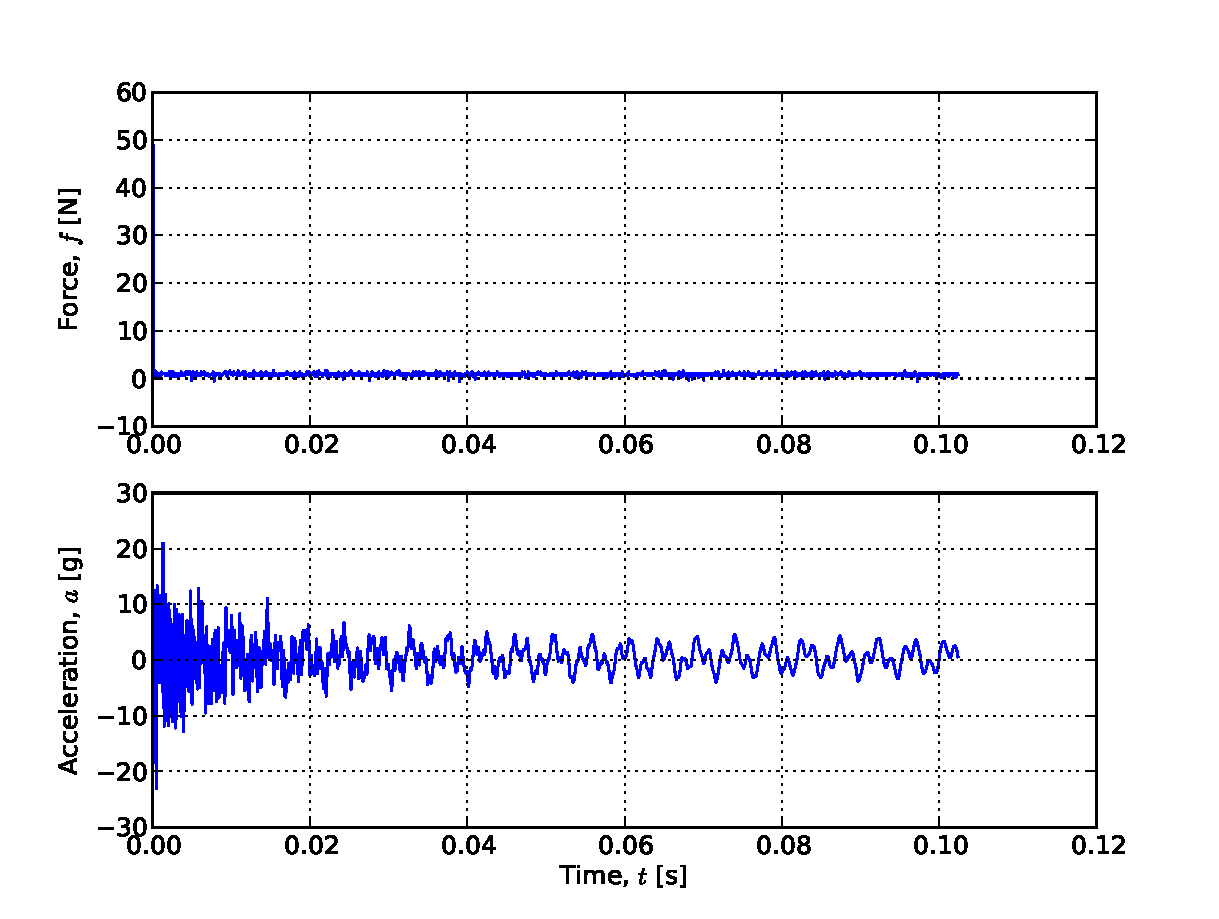
\includegraphics[width=.9\textwidth]{../Example_code/flex_vib.pdf}
\end{frame}

\begin{frame}{Vibration d'une cloche (salle C114)}
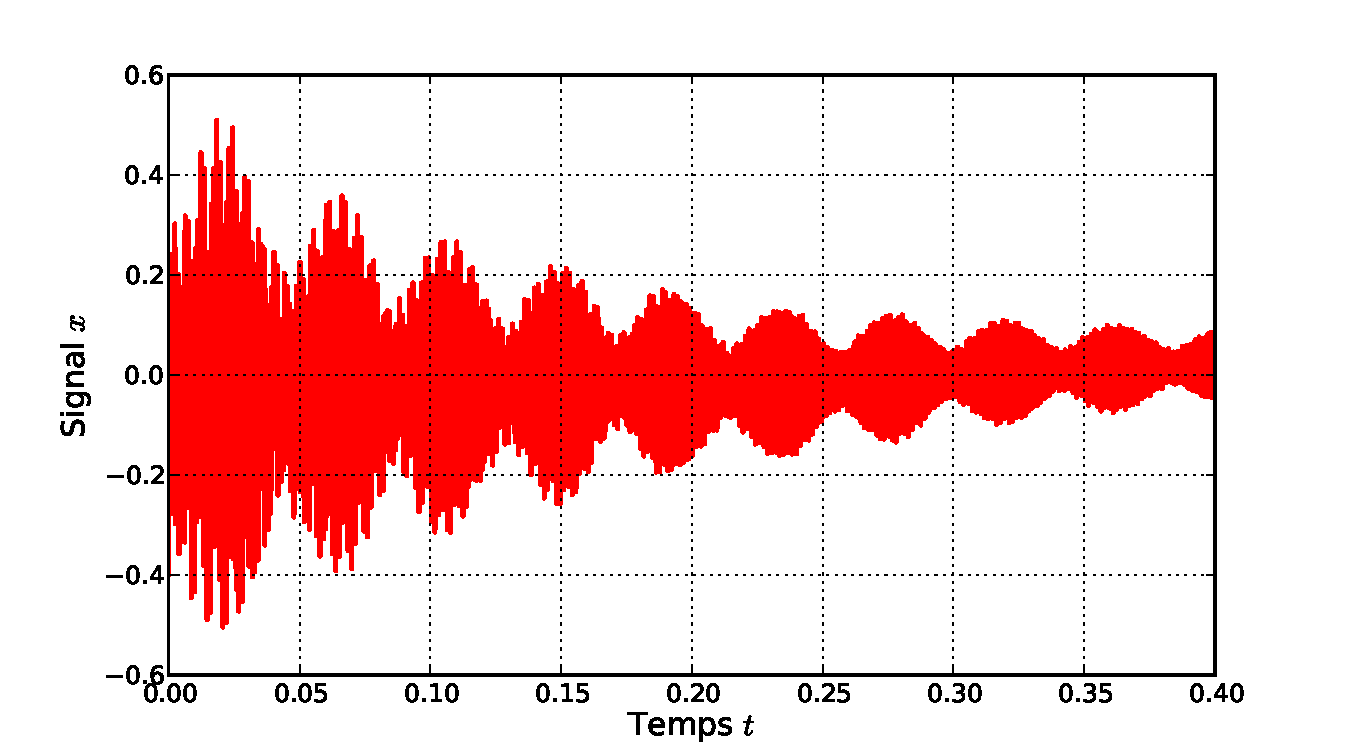
\includegraphics[width=.9\textwidth]{figures/cloche.pdf}
\end{frame}


\section{Notations}
\begin{frame}{Notations}
\begin{block}{Un signal ?}
Dans ce cours on étudie le comportement d'un signal $x$ issu de la mesure d'une grandeur physique (vitesse, température, \ldots). Le signal dépend d'une variable unique $t$ qui peut représenter le temps, une position \ldots 
\end{block}

\begin{block}{Signal quelconque}
D'un point de vue mathématique, le signal $x(t)$ défini par:
$$
x:t \longmapsto x(t), \; \forall x \in [0,t_{max}]
$$

\end{block}

\begin{block}{Signal périodique}
Si $x$ est périodique, on note $T$ sa période et $f$ sa fréquence avec:
$$
f = \frac{1}{T}
$$
\end{block}
\end{frame}

%\section{Outils}
%  \subsection{Python, c'est quoi ?}
%  \begin{frame}{Python, c'est quoi ?}
%  \begin{block}{Pourquoi Python ?}
%  \begin{itemize}
%  \item La lourdeur des calculs nécessite des outils numériques.
%  \item Les signaux expérimentaux sont numérisés et donc aisément traités par ces outils.
%  \item Python est un langage simple, au spectre d'applications vaste.
%  \item Python est libre et donc gratuit, vous pouvez donc l'installer rapidement sur toute machine. Il est présent sur la majorité des distributions de Linux.
%  \item Pour l'installer et lire les documentations: \href{http://www.python.org/}{http://www.python.org/}
%  \item Modules utilisés: 
%  \begin{itemize}
%  \item Graphisme: \href{http://matplotlib.sourceforge.net/}{Matplotlib}
%  \item Calcul scientifique: \href{http://www.scipy.org/}{Scipy}
%  \item Calcul numérique: \href{http://numpy.scipy.org/}{Numpy}
%  \end{itemize}
%  \end{itemize}
%  \end{block}
%  \end{frame}
%  \subsection{Python: comment ça marche ?}
%  
%  
%  
%  \begin{frame}[containsverbatim]
%  \frametitle{Python: comment ça marche ?}
%  \begin{block}{Outils nécessaires}
%  \begin{itemize}
%  \item Un éditeur de texte reconnaissant la syntaxe.
%  \item Un terminal.
%  \end{itemize}
%  \end{block}
%  \begin{block}{Exemple}
%  On crée un fichier \lstinline!test.py! dont le contenu est (voir dossier  \lstinline!/listings!):    
%  \lstinputlisting{listings/test.py}
%  On execute Python dans un terminal avec une des commandes suivantes:
%  \begin{lstlisting}
%  python test.py
%  \end{lstlisting}
%  Ou:
%  \begin{lstlisting}
%  python 
%  execfile(test.py)
%  \end{lstlisting}
%  La seconde solution a l'intérêt de ne pas fermer l'interpréteur après l'exécution ce qui permet de débugger ou de modifier le code plus aisément.
%  \end{block}
%  \end{frame}

%\section{Signaux}
%  \subsection{Signal sinusoïdal}
%  
%  \begin{frame}[containsverbatim]
%  \frametitle{Signal sinusoïdal (1/3)}
% \begin{block}{Définition} 
% \lstinputlisting{listings/signal_sinusoidal.py}
% \end{block}
%  
%  \begin{block}{Fonction de tracé} 
%  On construit une fonction qui assure le tracé:
%  \lstinputlisting{listings/trace_signal.py}
%  \end{block}
%  \end{frame}
%  
%  \begin{frame}[containsverbatim]
%  \frametitle{Signal sinusoïdal (2/3)}
%  \begin{block}{Tracé du signal} 
%  \lstinputlisting{listings/exemple1.py}
%  \end{block}
%  \end{frame}
%  
%  \begin{frame}[containsverbatim]
%  \frametitle{Signal sinusoïdal (3/3)}
%  On obtient le fichier (vectoriel) \lstinline!sinusoide.pdf!\\  
%  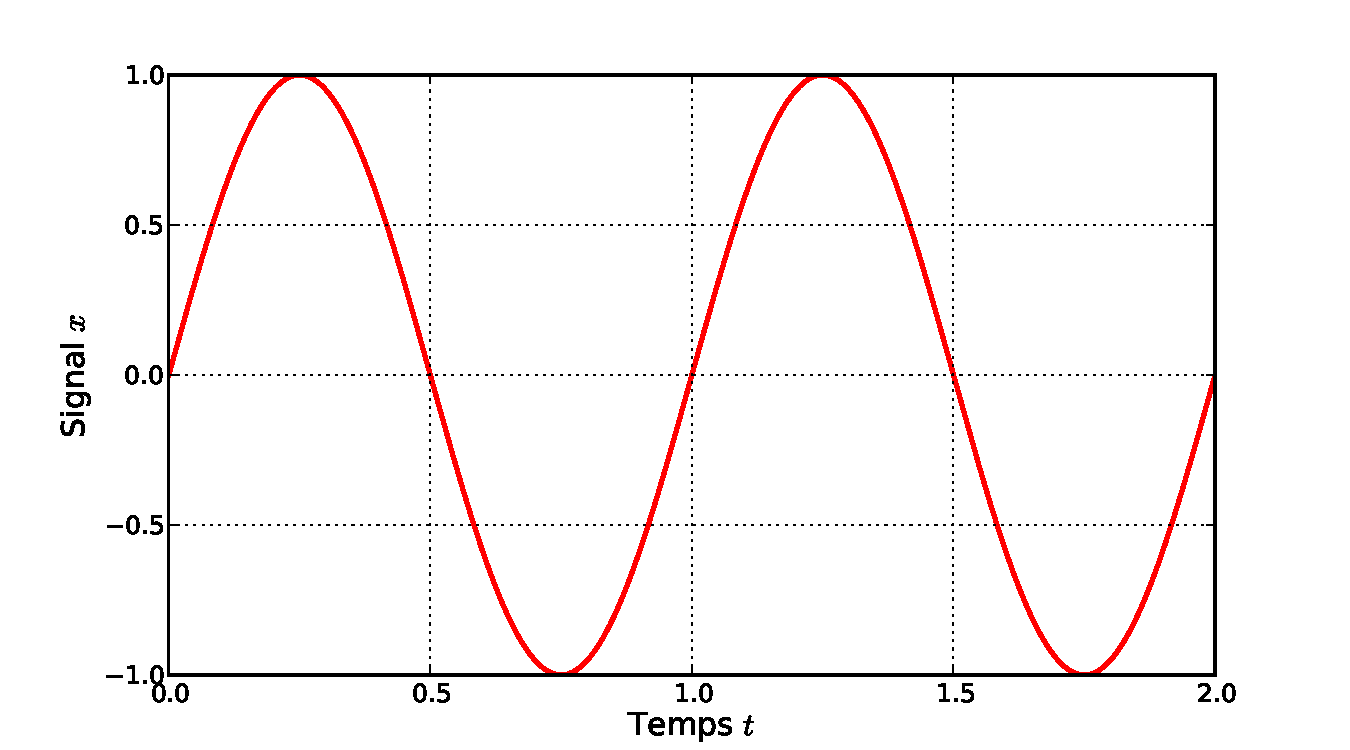
\includegraphics[width=1.\textwidth]{figures/sinusoide.pdf}
%  \end{frame}
%  
%  
%%  \subsection{Signal bisinusoïdal}
%%  \begin{frame}[containsverbatim]
%%  \frametitle{Signal bisinusoïdal (1/2)}
%%  \begin{block}{Intérêt}
%%  Ce signal est la somme de deux composantes sinusoïdales pures. Il permet la mise en évidence des interactions entre les deux composantes lors du traitement.
%%  \end{block}
%%  \begin{block}{Tracé}
%%  \lstinputlisting{listings/exemple3.py}
%%  \end{block}  
%%  \end{frame}  
%  
%%  \begin{frame}{Signal bisinusoïdal (2/2)}
%%  On obtient le fichier (vectoriel) \lstinline!bisinus.pdf!\\  
%%  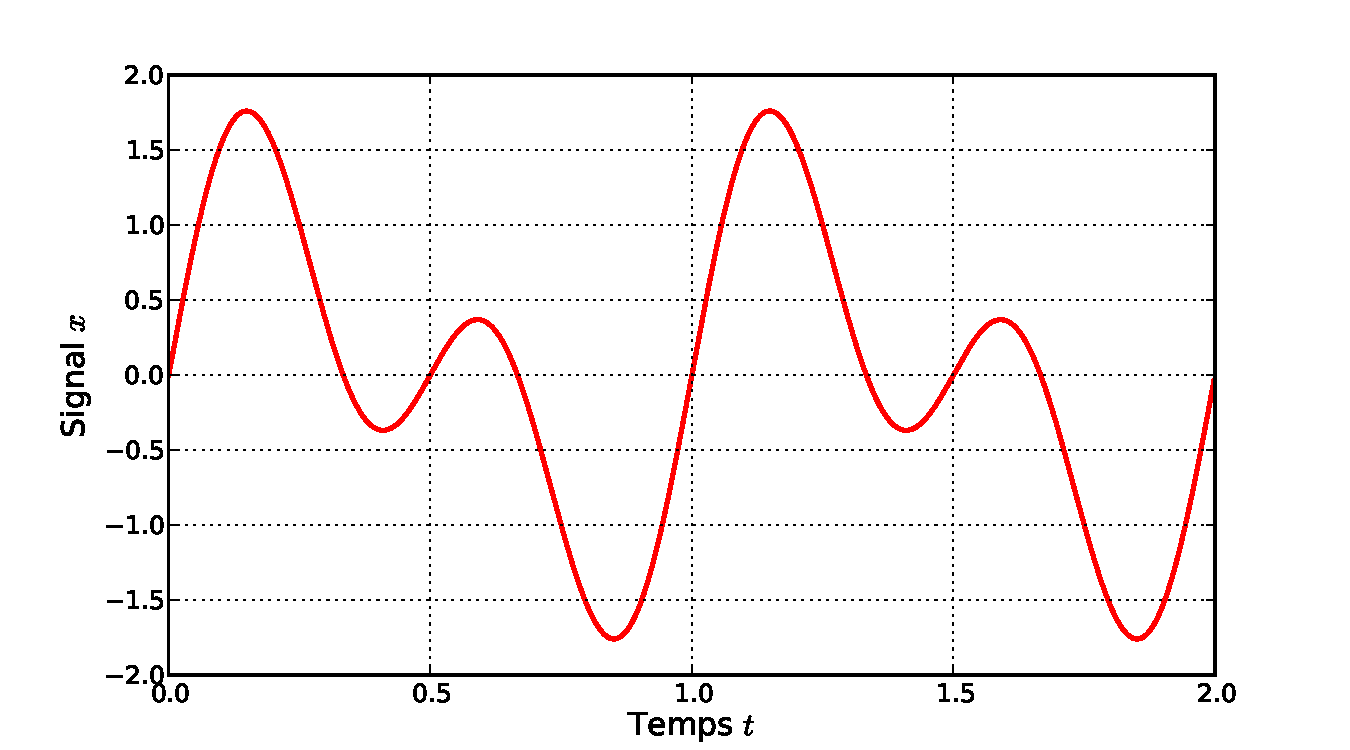
\includegraphics[width=1.\textwidth]{figures/bisinus.pdf}
%%  \end{frame}  
%  
%  \subsection{Signal carré}
%  \begin{frame}[containsverbatim]
%  \frametitle{Signal carré (1/3)}
%  \begin{block}{Construction de la fonction} 
%  \lstinputlisting{listings/signal_carre.py}
%  \end{block}
%  \end{frame}  
%  
%  \begin{frame}[containsverbatim]
%  \frametitle{Signal carré (2/3)}  
%  \begin{block}{Tracé du signal} 
%  \lstinputlisting{listings/exemple2.py}
%  \end{block}
%  \end{frame}
%  \begin{frame}[containsverbatim]
%  \frametitle{Signal carré (3/3)}
%  On obtient le fichier (vectoriel) \lstinline!carre.pdf!\\  
%  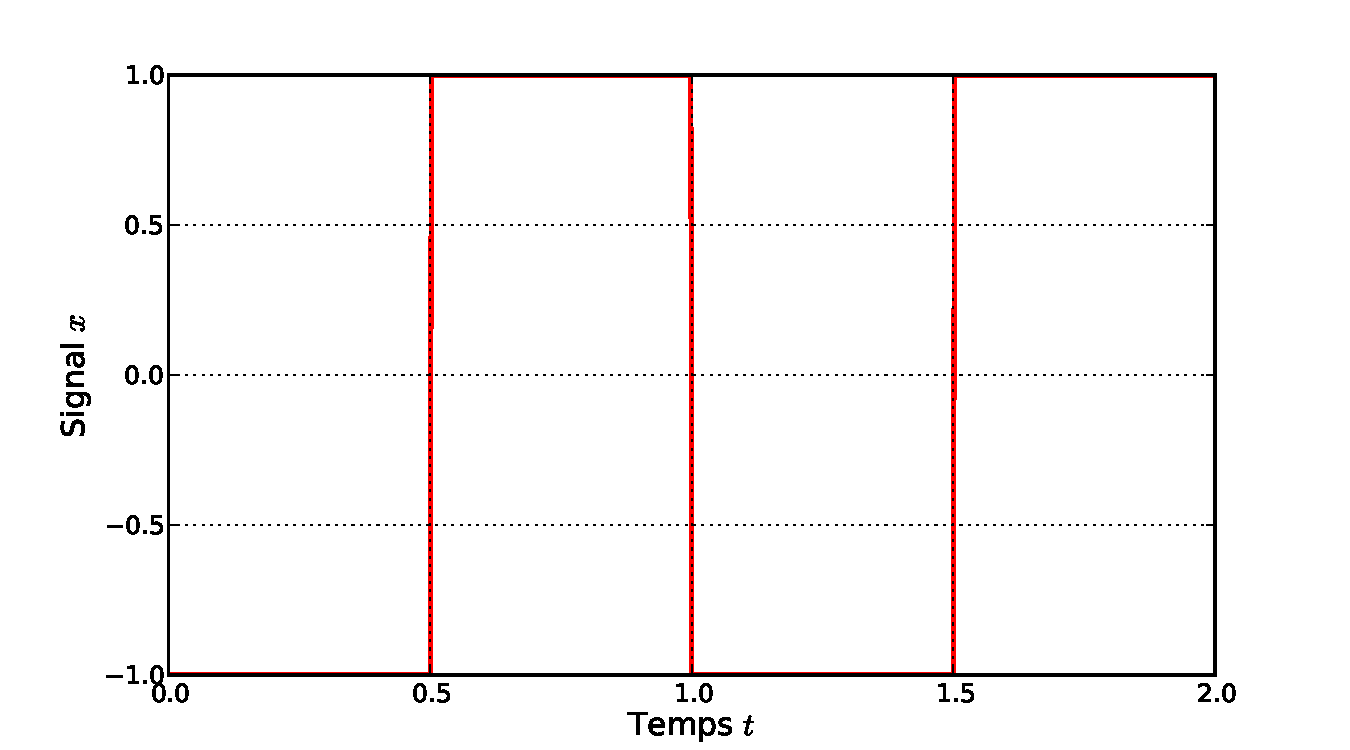
\includegraphics[width=1.\textwidth]{figures/carre.pdf}
%  \end{frame}
%  
%  \subsection{Signal expérimental: mesure d'accélération sur une cloche}
%  \begin{frame}[containsverbatim]
%  \frametitle{Signal expérimental: mesure d'accélération sur une cloche}
%  \begin{block}{Intérêt}
%  Ce signal pseudo périodique est obtenu expérimentalement au moyen d'un accéléromètre fixé sur une cloche (visible en salle C114) et excitée par un battant. Il est fourni dans une fichier sérialisé par le module Python \href{http://docs.python.org/library/pickle.html}{Pickle}.  
%  \end{block}
%  \begin{block}{Tracé}
%  \lstinputlisting{listings/exemple4.py}
%  \end{block}
%  \end{frame}
%  \begin{frame}[containsverbatim]
%  \frametitle{Signal expérimental: mesure d'accélération sur une cloche}
%  On obtient le fichier (vectoriel) \lstinline!cloche.pdf!\\  
%  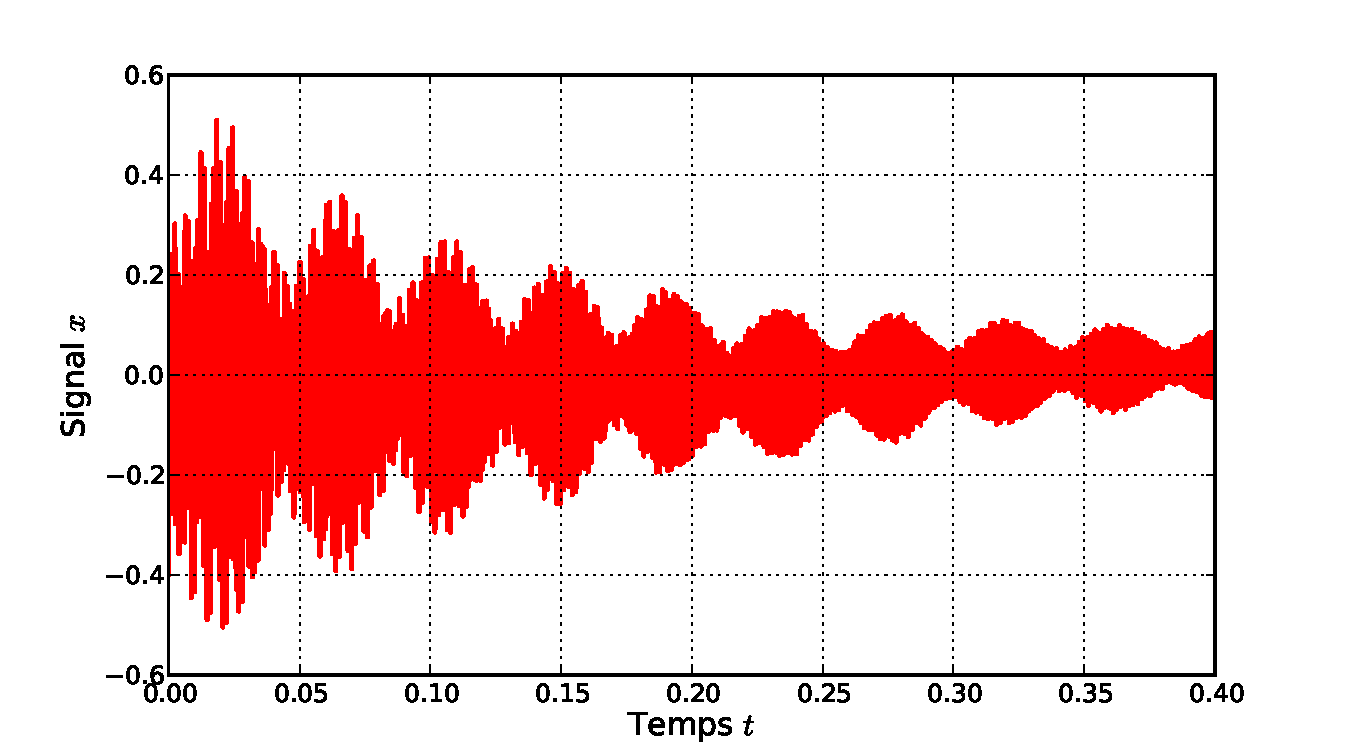
\includegraphics[width=1.\textwidth]{figures/cloche.pdf}
%  \end{frame}

\section{Échantillonnage}
  \subsection{Les bases}
  \begin{frame}{Les bases}
  \begin{block}{Principe}
  \'Echantilloner un signal $x$ consiste à l'évaluer sur une grille comportant $N$ points définie par:
  $$
  t_n = t_{min}+\frac{n}{f_e}, \; n \in \; [0,N[
  $$
  La fréquence $f_e$ est la fréquence échantillonnage. La durée d'observation du signal notée $D$ est donc obtenue par:
  $$
  D = N/f_e
  $$
  Le signal échantillonné est alors obtenu par:
  $$
  x_n=x(t_n)
  $$
  On note $[t_n]$ et $[x_n]$ les vecteurs ainsi obtenus.
  \end{block}
  \begin{block}{Paramètres importants}  
  \begin{itemize}
  \item $\frac{D}{T}$: ajustable en modifiant la durée d'observation $D$
  \item $\frac{f_e}{f}$: ajustable en modifiant la fréquence d’échantillonnage $f_e$.
  \end{itemize}
  \end{block}
  \end{frame}
  
  \subsection{Choix de la durée d'observation}
  \begin{frame}{Choix de la durée d'observation (1/2)}
  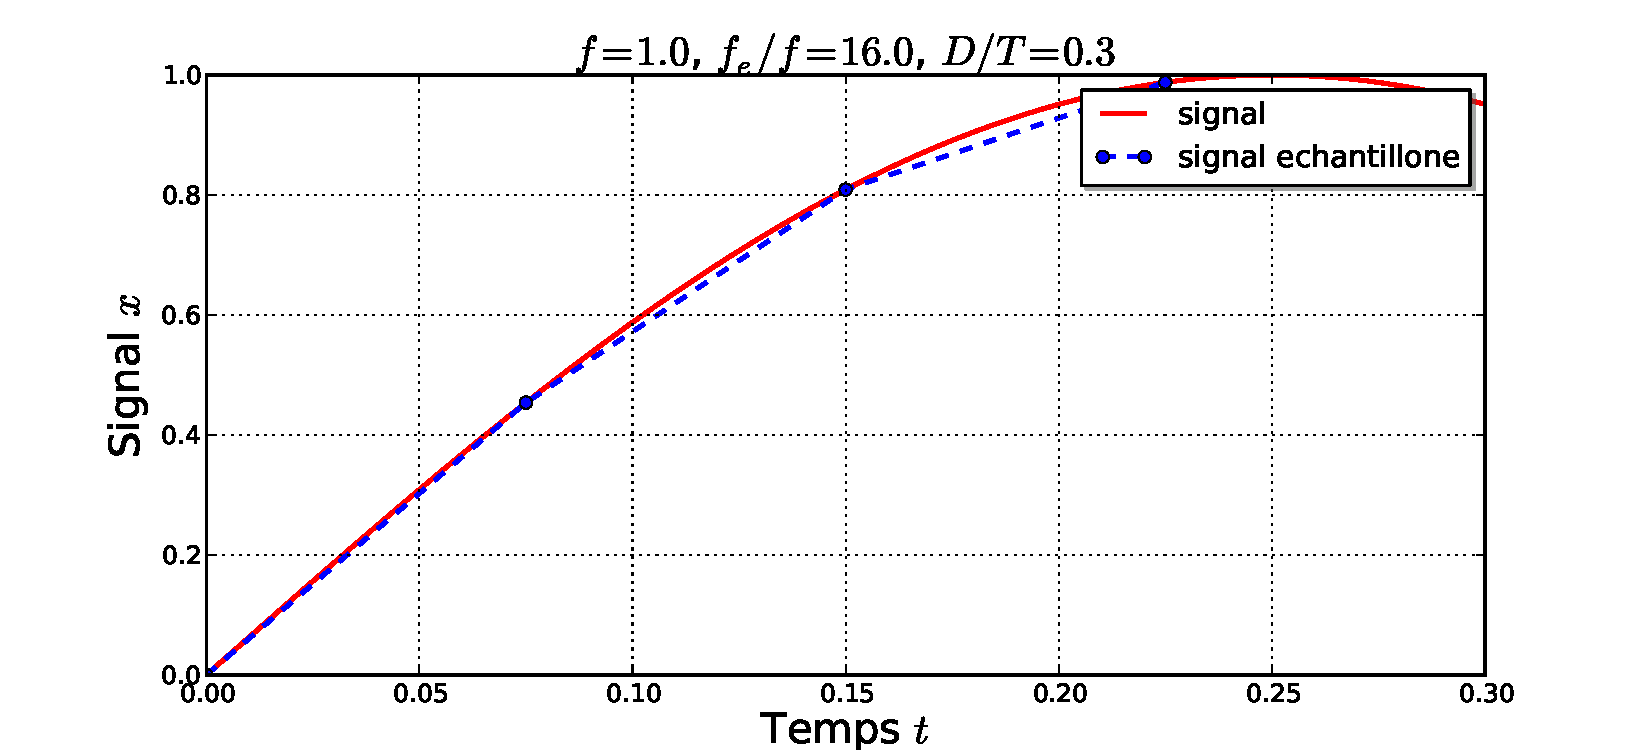
\includegraphics[width=1.\textwidth]{figures/echant_sin_3.pdf}\\
  \alert{Temps d'observation $D$ trop court !}
  \end{frame}
  \begin{frame}{Choix de la durée d'observations (2/2)}
  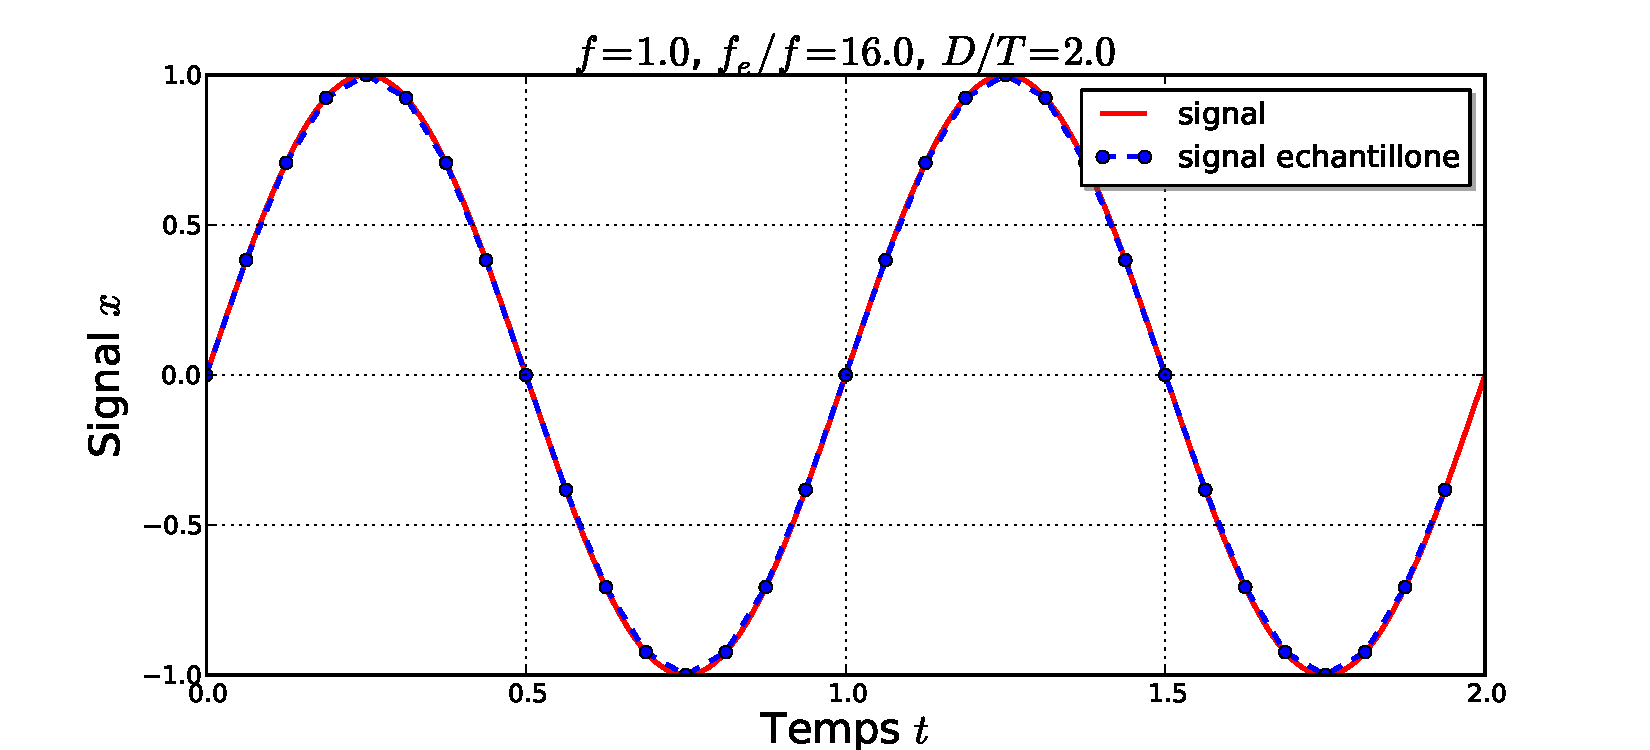
\includegraphics[width=1.\textwidth]{figures/echant_sin_0.pdf}\\
  \begin{alertblock}{Conclusion}
  \begin{itemize}
  \item Il faut que $D/T \geq 1$ 
  \item Idéalement, $D/T \in \bf N$
  \end{itemize}
  \end{alertblock}
  \end{frame}
  \subsection{Une borne basse de la fréquence d'échantillonage ?}
  \begin{frame}{Une borne basse de la fréquence d'échantillonage ?}
  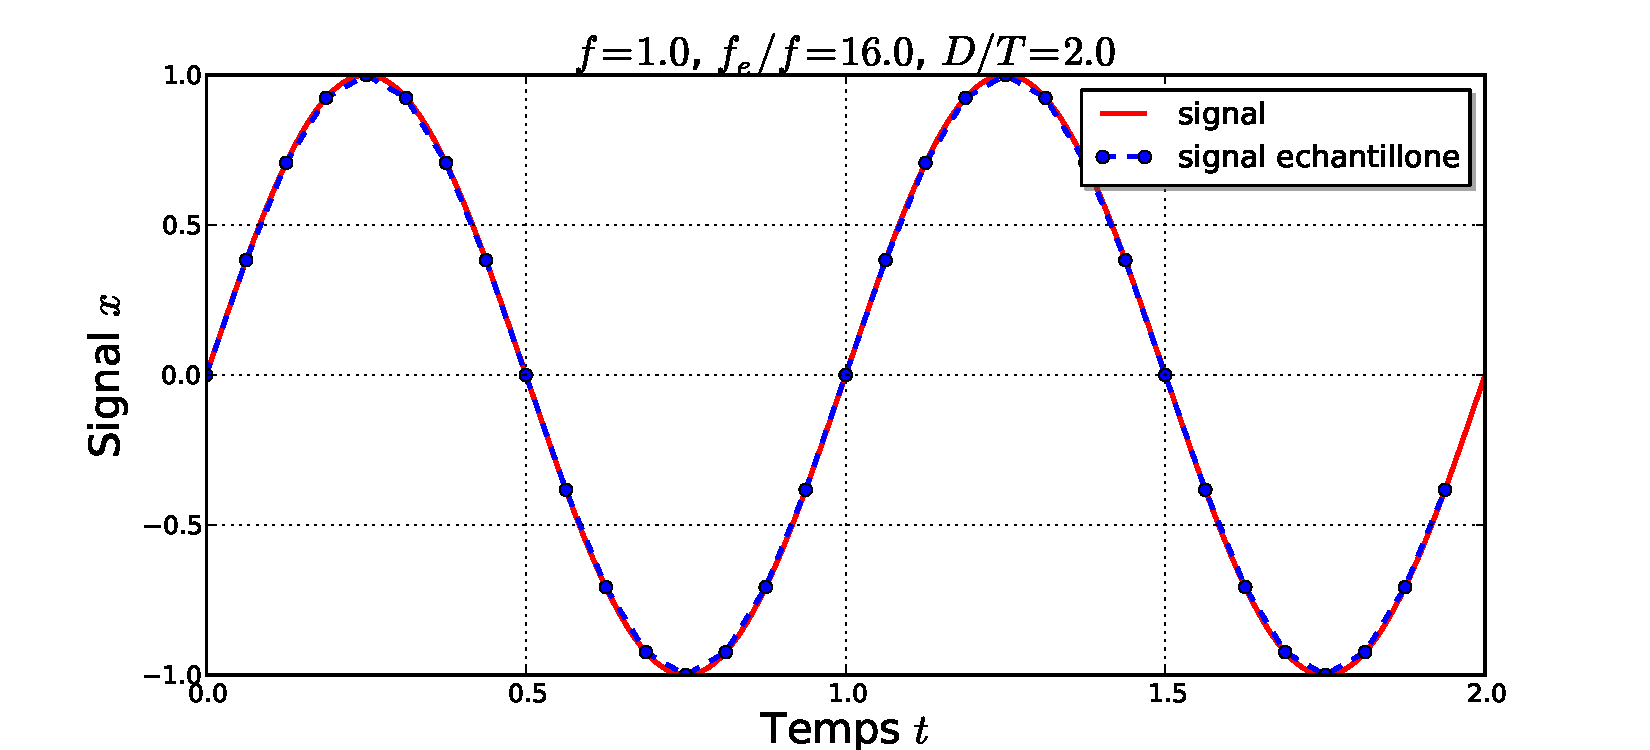
\includegraphics[width=1.\textwidth]{figures/echant_sin_0.pdf}\\
  \'Echantillonage correct.
  \end{frame}
  \begin{frame}{Une borne basse de la fréquence d'échantillonage ?}
  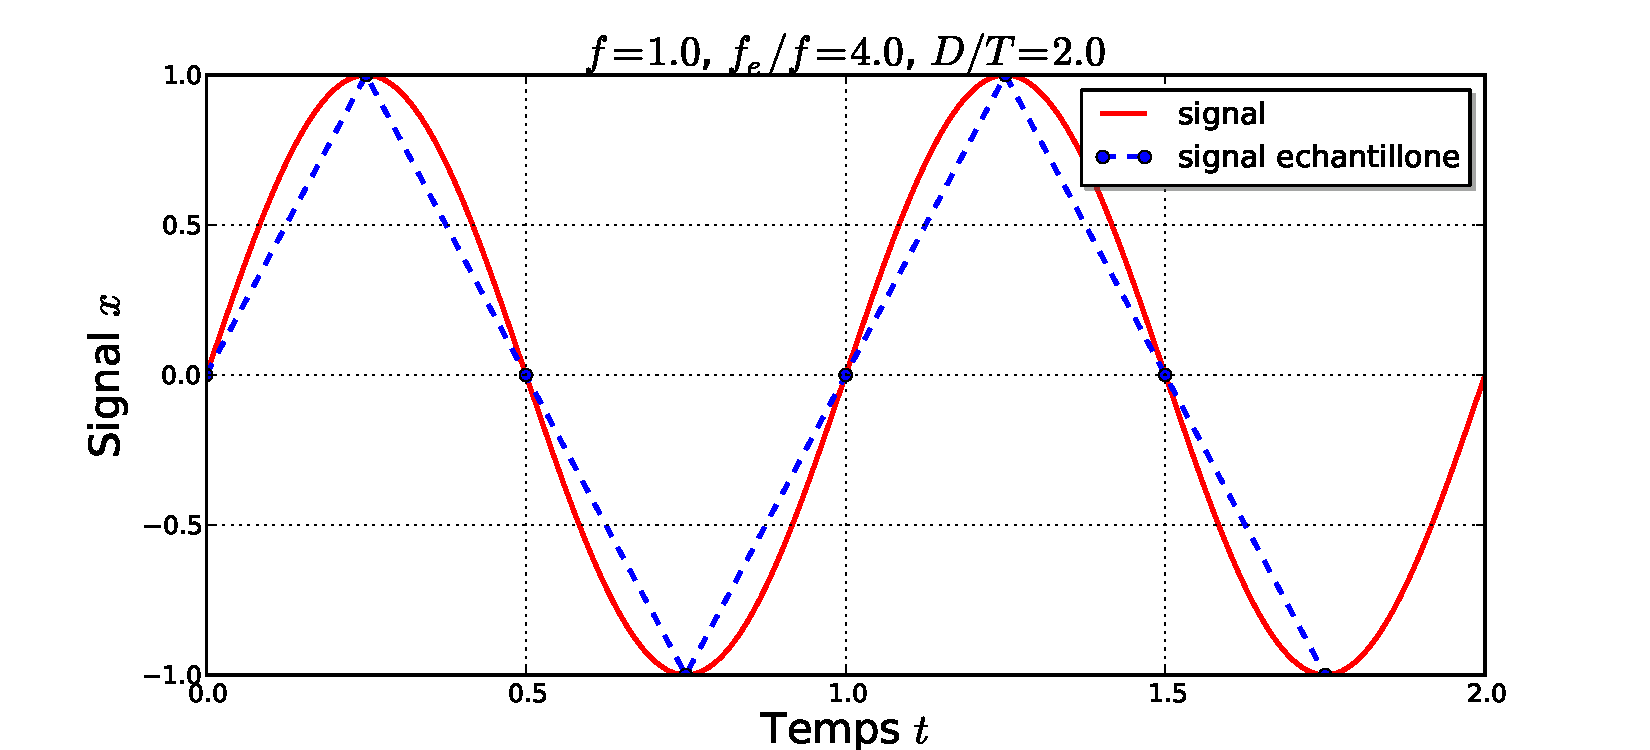
\includegraphics[width=1.\textwidth]{figures/echant_sin_1.pdf}\\
  \'Echantillonage correct.
  \end{frame}
  \begin{frame}{Une borne basse de la fréquence d'échantillonage ?}
  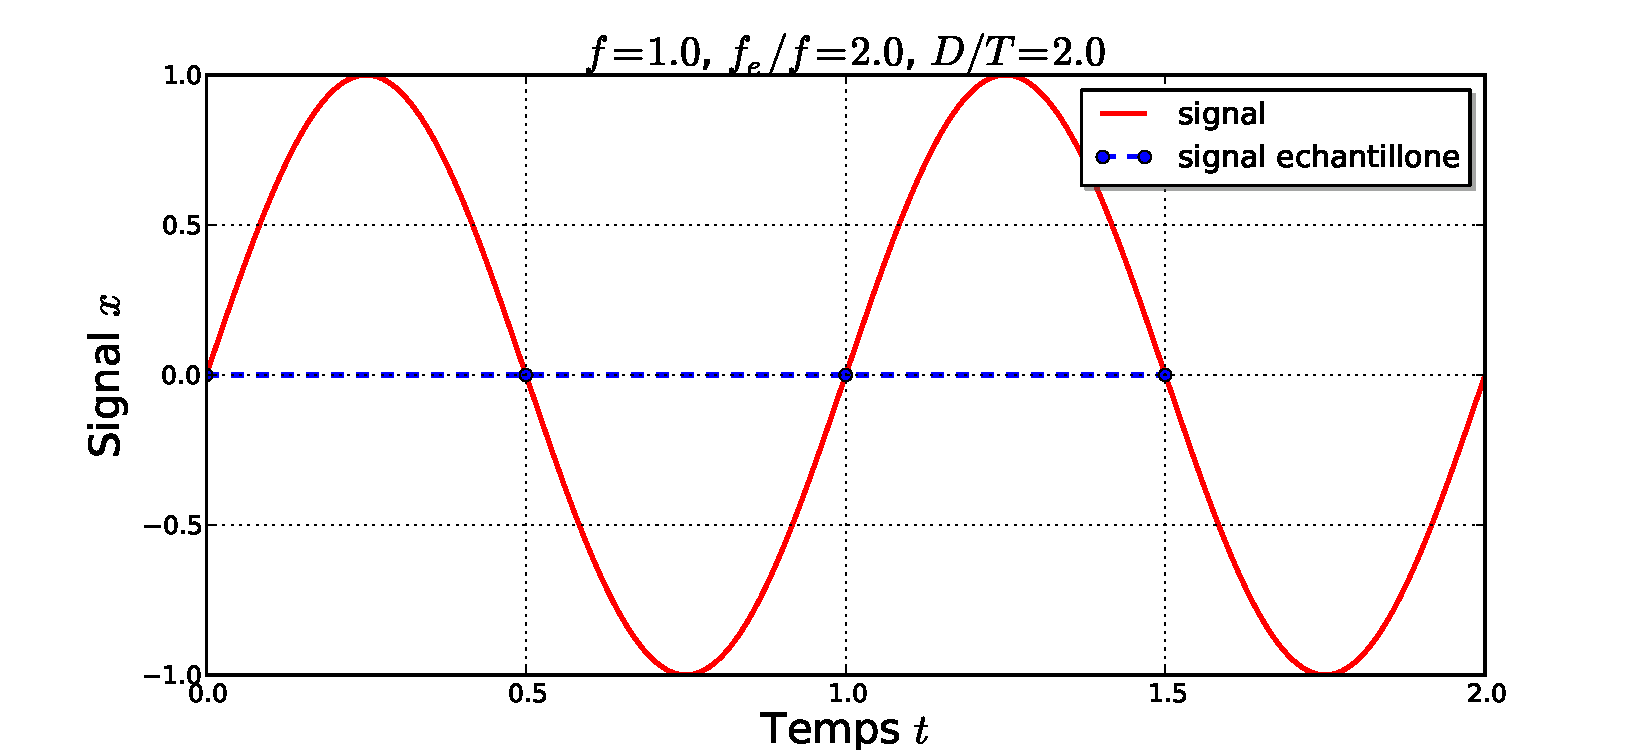
\includegraphics[width=1.\textwidth]{figures/echant_sin_5.pdf}\\
  \alert{Fréquence d'échantillonage trop basse.}
  \end{frame}
  \begin{frame}{Borne basse de la fréquence d'échantillonage ?}
  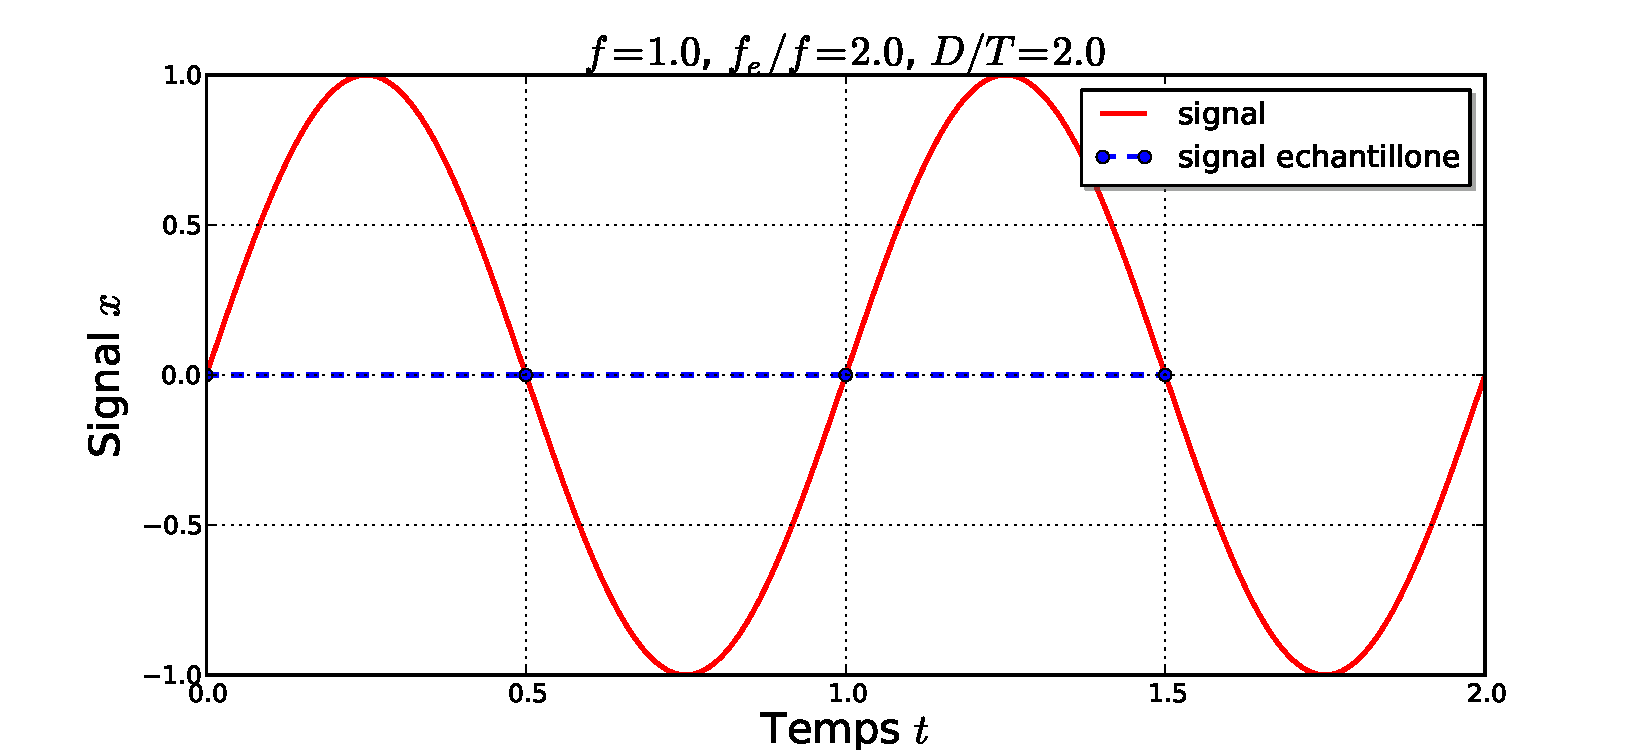
\includegraphics[width=1.\textwidth]{figures/echant_sin_2.pdf}\\
  \alert{Fréquence d'échantillonage $f_e$ trop basse.}
  \begin{alertblock}{Bilan: le théorème de Shannon-Nyquist}
  Toute composante du signal dont la fréquence est supérieure ou égale à $f_e/2$ sera perdue lors de l'échantillonage.
  \end{alertblock}
  \end{frame}
  \subsection{Hautes fréquences et aliasing}
  \begin{frame}{Hautes fréquences et aliasing}
  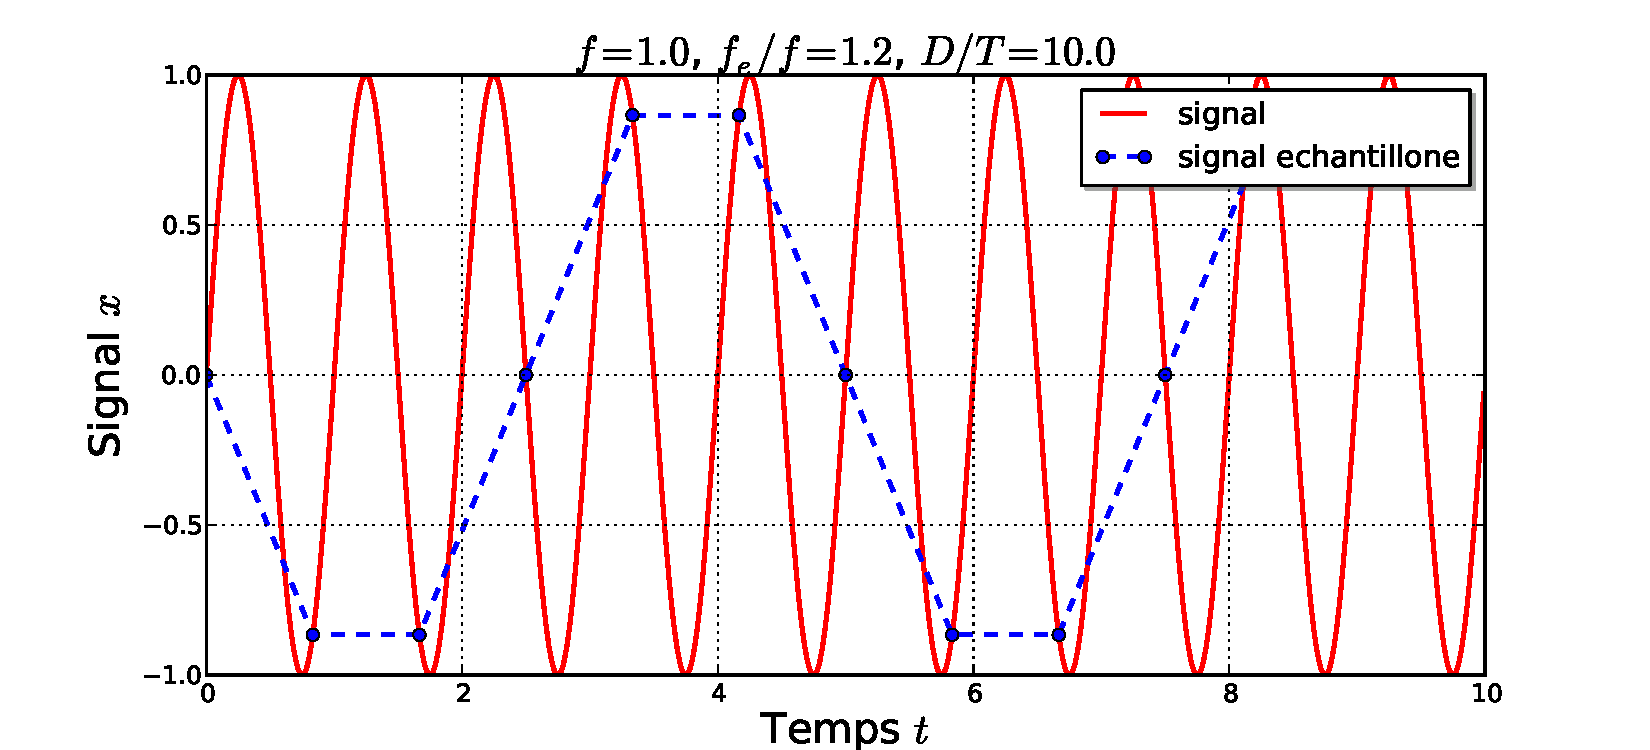
\includegraphics[width=1.\textwidth]{figures/echant_sin_6.pdf}\\
  \begin{alertblock}{Hautes fréquences et aliasing}
  Les fréquences trop hautes vis-à-vis de la fréquence d’échantillonnage (\textit{i. e.} $f\geq f_e/2$) sont non seulement perdues mais peuvent produire des artefacts sous la forme de basses fréquences. Il est donc impératif de filtrer le signal préalablement à son échantillonnage pour couper toutes les fréquences supérieures à $f_e/2$.
  \end{alertblock}
  \end{frame}

  
  \begin{frame}{Hautes fréquences et aliasing}
  
  \begin{block}{Explication mathématique}
  Intéressons nous aux signaux de fréquence $f^*=f+k f_e$ avec $k\in \mathbb{Z}$. On les échantillonne:
  \begin{align}
  x_n^* & = \sin(2\pi \frac{f^*}{f_e}n) \nonumber \\
  & = \sin(2\pi \frac{f+k f_e}{f_e}n) \nonumber \\ 
  & = \sin(2\pi n k + 2\pi \frac{f}{f_e}n) \nonumber \\ 
  & = \sin(2\pi \frac{f}{f_e}n) \nonumber \\
  & = x_n \nonumber
  \end{align}
  \end{block}
  \begin{alertblock}{Ce qu'il faut comprendre}
  Les signaux de fréquence $f^*=f+k f_e$ avec $k\in \mathbb{Z}$ sont indiscernables par échantillonnage. Dans le cadre d'une étude expérimentale, il faut donc s'assurer qu'une seule de ces fréquences est présente dans le signal échantillonné.
  \end{alertblock}
  \end{frame}
  
  \begin{frame}[containsverbatim]
  \frametitle{Mises en pratique (1/2)}
  \lstinputlisting{listings/exemple_aliasing.py}
  \end{frame}
  
  \begin{frame}{Mises en pratique (2/2)}
  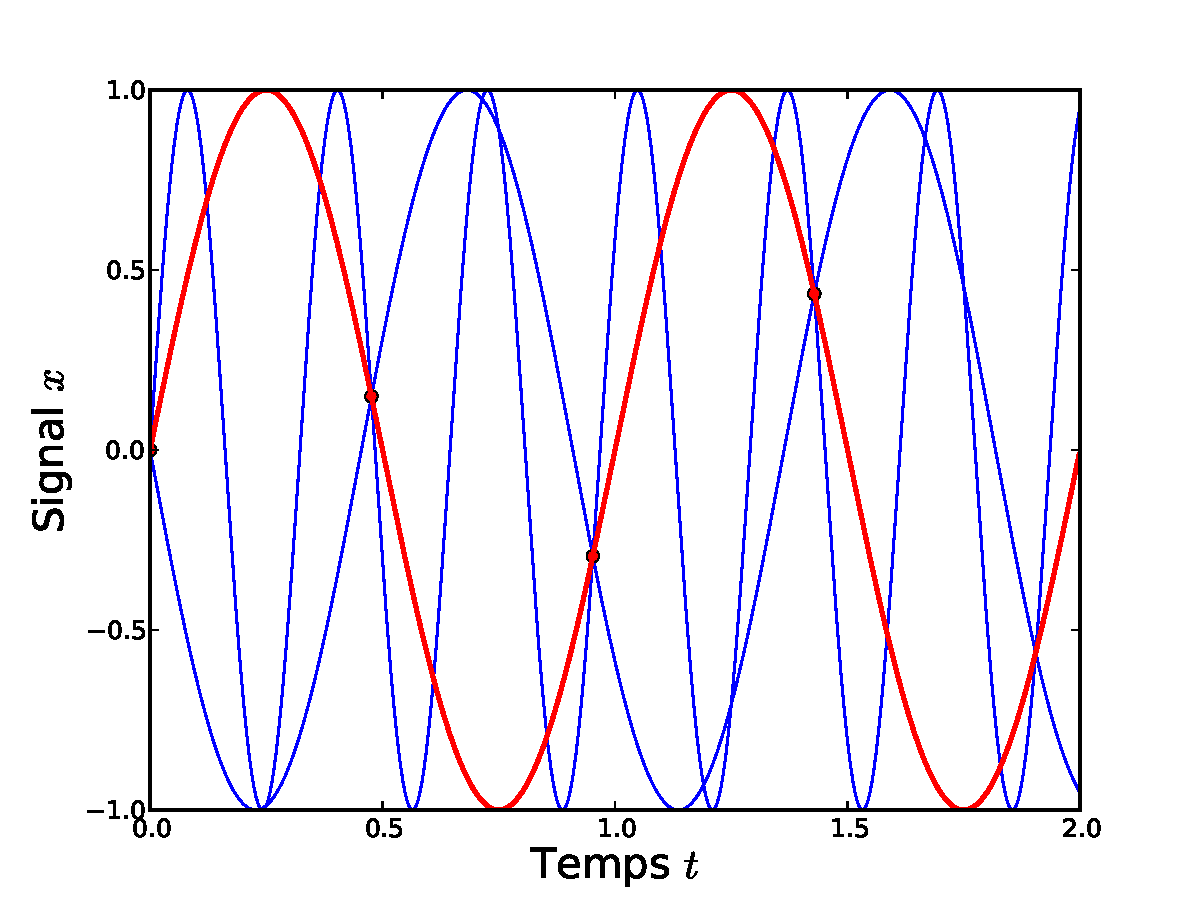
\includegraphics[width=.9\textwidth]{figures/exemple_aliasing.pdf}\\
  \end{frame}
  
\section{Analyse fréquentielle}
\begin{frame}{Décomposition des signaux périodiques}
\begin{block}{Fonctions de base}
On peut projeter les signaux de fréquence $f$ sur une base de dimension infinie constituée de fonctions de la forme:
$$
f_n(t)=sin(2\pi n f t)\mbox{ et } g_n(t)=\cos(2\pi n f t)
$$ 
\end{block}
\begin{block}{Décomposition sur la base}
Un signal périodique $x(t)$ peut donc s'écrire sous la forme:
$$
x(t) = \sum\limits_{n=0}^{+\infty} a_n sin(2\pi n f t) + b_n \cos(2\pi n f t)
$$
\end{block}
\begin{alertblock}{Points essentiels}
\begin{itemize}
\item Connaître $[a_n]$ et $[b_n]$, c'est connaître $x(t)$ en tout point.
\item Cette décomposition donne une interprétation fréquentielle de $x(t)$.
\item La question est donc de savoir comment calculer analytiquement et numériquement $[a_n]$ et $[b_n]$.
\end{itemize}
\end{alertblock}

\end{frame}

\begin{frame}{Développement en séries de Fourier}
\begin{block}{Les grandes lignes}
\begin{itemize}
\item Les séries de Fourier permettent d'effectuer la projection des signaux périodiques sur la base $[f_n(t),g_n(t)]$ de manière analytique.
\item Quand $N$ tend vers l'infini, la somme converge vers le signal $x(t)$. 
\item Pour les signaux présentant des singularités (triangle, carré), elle converge plus lentement.
\end{itemize}
\end{block}
\begin{alertblock}{Formulation}
$$
\sum\limits_{n=-N}^{+N}c_n(x)e^{2j\pi n f t} \underset{N\to \infty}{\longrightarrow} x(t)
$$
Où les coefficients complexes $c_n(x)\in \mathbb{C}$ sont définis par:
$$
c_n(x)=\frac{1}{T}\int_{0}^{T}x(t)e^{-2j\pi n f t}dt\mbox{ avec: } T=\frac{1}{f}
$$
\end{alertblock}
\end{frame}

\begin{frame}{Exercices}
\begin{block}{Remarques et notations}
\begin{itemize}
\item $x(t)$, $y(t)$ et $z(t)$ sont des fonctions de période $T$ du temps $t$.
\item $\alpha$ est un nombre réel.
\item On pourra introduire la pulsation $\omega=2\pi f$ pour simplifier les calculs.
\item On rappelle que:
$$
\cos(a-b) = \cos(a)\cos(b)+\sin(a)\sin(b)\; ; \; \sin(a+b)=\sin(a)\cos(b)+\sin(b)\cos(a)
$$
$$
\cos(a) = \frac{e^{ja}+e^{-ja}}{2}\; ; \;\sin(a) = \frac{e^{ja}-e^{-ja}}{2j}
$$
\end{itemize}
\end{block}

\begin{block}{Pour chaque signal $x$, trouver l'ensemble des coefficients $c_n(x)$}
\begin{enumerate}
\item $x(t) = \cos (2\pi f t)$
\item $x(t) = \cos^2(2\pi ft)$
\item $x(t) = \alpha y(t)$
\item $x(t) = y(t)+z(t)$
\end{enumerate}
\end{block}
\end{frame}

\begin{frame}{Exercice: signal sinusoïdal}
\begin{block}{Réécriture}
\begin{align}
x(t) & = sin(2\pi ft) \nonumber \\
& = \frac{e^{2j\pi ft}- e^{-2j\pi ft}}{2j} \nonumber\\
& = \frac{j}{2}e^{-2i\pi ft} -\frac{j}{2}e^{2j\pi ft} \nonumber
\end{align}
\end{block}
\begin{alertblock}{Coefficients}
$$
c_n(x) = \left\{
\begin{split}
-\frac{j}{2}\mbox{ si: }n=1\\
\frac{j}{2}\mbox{ si: }n=-1\\
0 \; \forall\;  n \;\in \;\mathbb{Z} -\left\{1,-1\right\} 
\end{split}
\right.
$$
\end{alertblock}
\end{frame}



\begin{frame}{Interprétation des coefficients $c_n$}
\begin{block}{Comment passer de $[c_n]$ à $[a_n,b_n]$}
On note $\Re$ la fonction partie réelle et $\Im$ la fonction partie imaginaire. On remarque que dans le cas des signaux à valeurs réels (ce qui est majoritairement le cas en physique):
$$
c_{-n} = \Re(c_n)-j\Im(c_n)= \overline c_n
$$
Les coefficients associés à $n<0$ sont donc inutiles car conjugués de coefficients obtenus pour $n>=0$. On remarque aussi que les coeffients $a_n$ et $b_n$ peuvent être calculés pour $n\geq0$:
\begin{align}
a_n = 2\Re(c_n) \nonumber\\
b_n = -2\Im(c_n)\nonumber
\end{align}


\end{block}
\end{frame}

\begin{frame}{Exercice: signal carré}
\begin{block}{Calculs}
$$
x(t) = \left\{
\begin{split}
-1 \mbox{ si: } t \in ]0,T/2[\\
1 \mbox{ si: } t \in ]T/2,T[
\end{split}
\right. 
$$
Donc:
\begin{align}
c_n(x) & = \frac{1}{T}\int_{0}^{T}x(t)e^{-2j\pi n f t}dt \nonumber \\
& = -\frac{1}{T}\int_{0}^{T/2}e^{-2j\pi n f t}dt+\frac{1}{T}\int_{T/2}^{T}e^{-2j\pi n f t}dt \nonumber \\
& = \frac{1}{T}\left(   \left[ \frac{-j}{2\pi nf} e^{-2j\pi n f t} \right]_0^{T/2} + \left[ \frac{j}{2\pi nf} e^{-2j\pi n f t} \right]_{T/2}^T \right)\nonumber
\end{align}
\end{block}
\begin{alertblock}{Coefficients}
$$
c_n(x)=-j\frac{2}{\pi n}\mbox{ avec: } n=2k+1\mbox{ et: }k\in\mathbb{Z}
$$
\end{alertblock}
\end{frame}



%\begin{frame}{Représentation des coefficients $c_n$}
%\begin{block}{Trace des coefficients}
%\lstinputlisting{listings/trace_complexes.py}
%\end{block}
%\end{frame}



\begin{frame}[containsverbatim]
  \frametitle{Exercice: signal carré}
\begin{block}{Mise en pratique: voyons si ça marche}
\lstinputlisting{listings/serieF_carre.py}
\end{block}
\end{frame}

\begin{frame}[containsverbatim]
  \frametitle{Exercice: signal carré}
\begin{block}{Programme de tracé de vecteurs complexes}
\lstinputlisting{listings/trace_complexes.py}
\end{block}
\end{frame}

\begin{frame}{Exercice: signal carré}
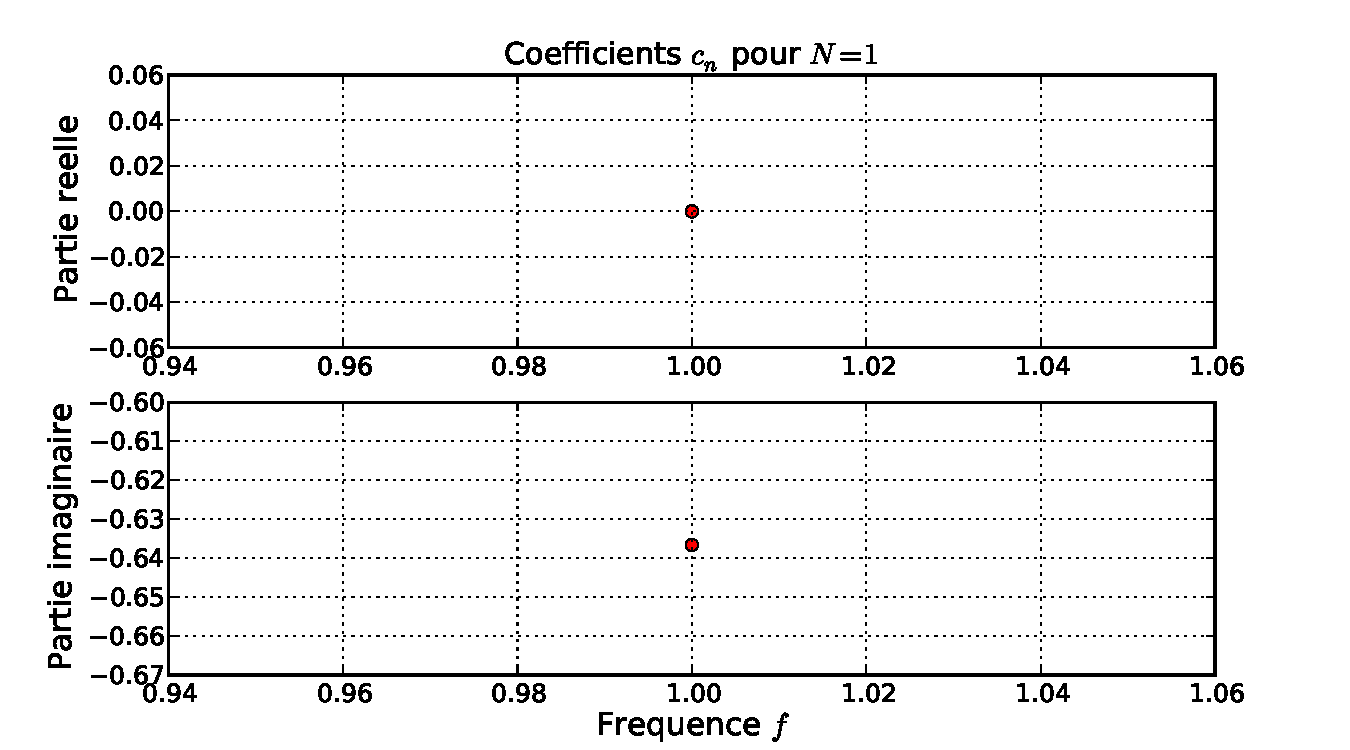
\includegraphics[width=1.\textwidth]{figures/serieF_carre_c_1.pdf} \\
\end{frame}

\begin{frame}{Exercice: signal carré}
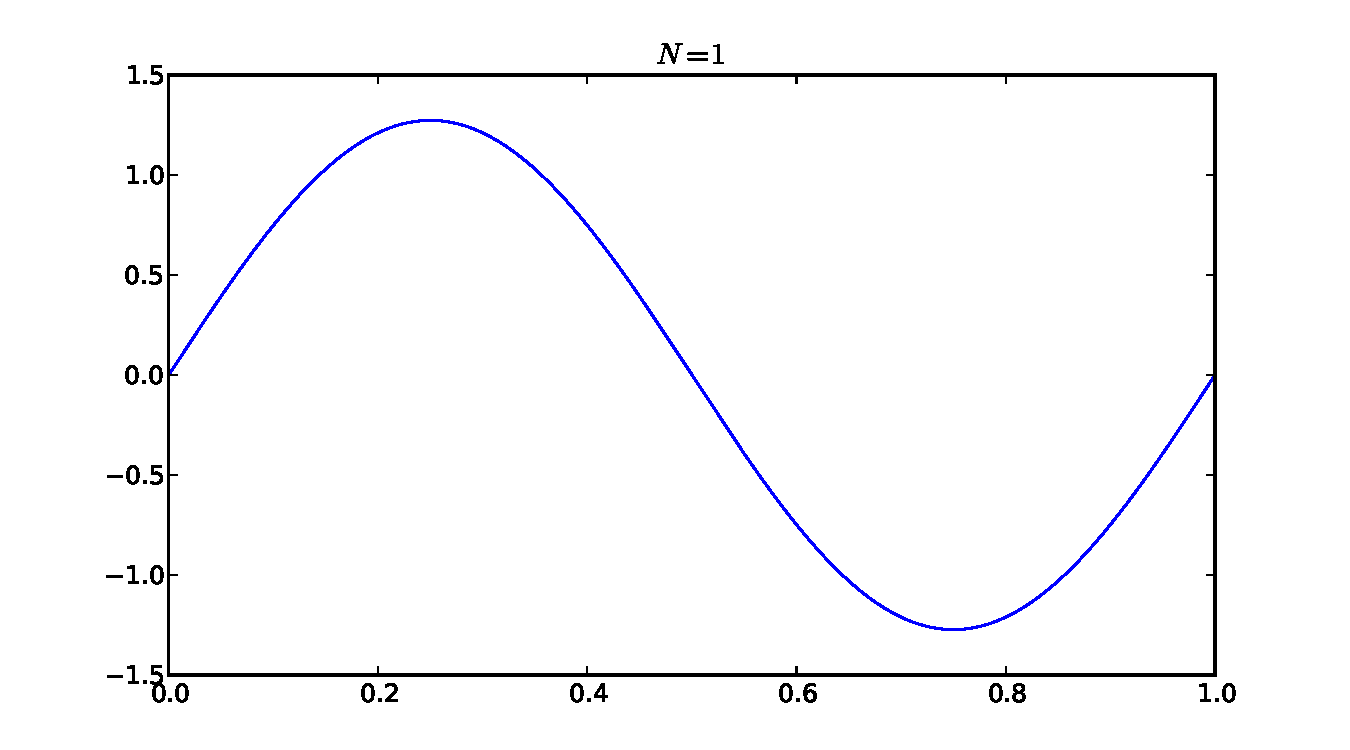
\includegraphics[width=1.\textwidth]{figures/serieF_carre_1.pdf}\\
\end{frame}

\begin{frame}{Exercice: signal carré}
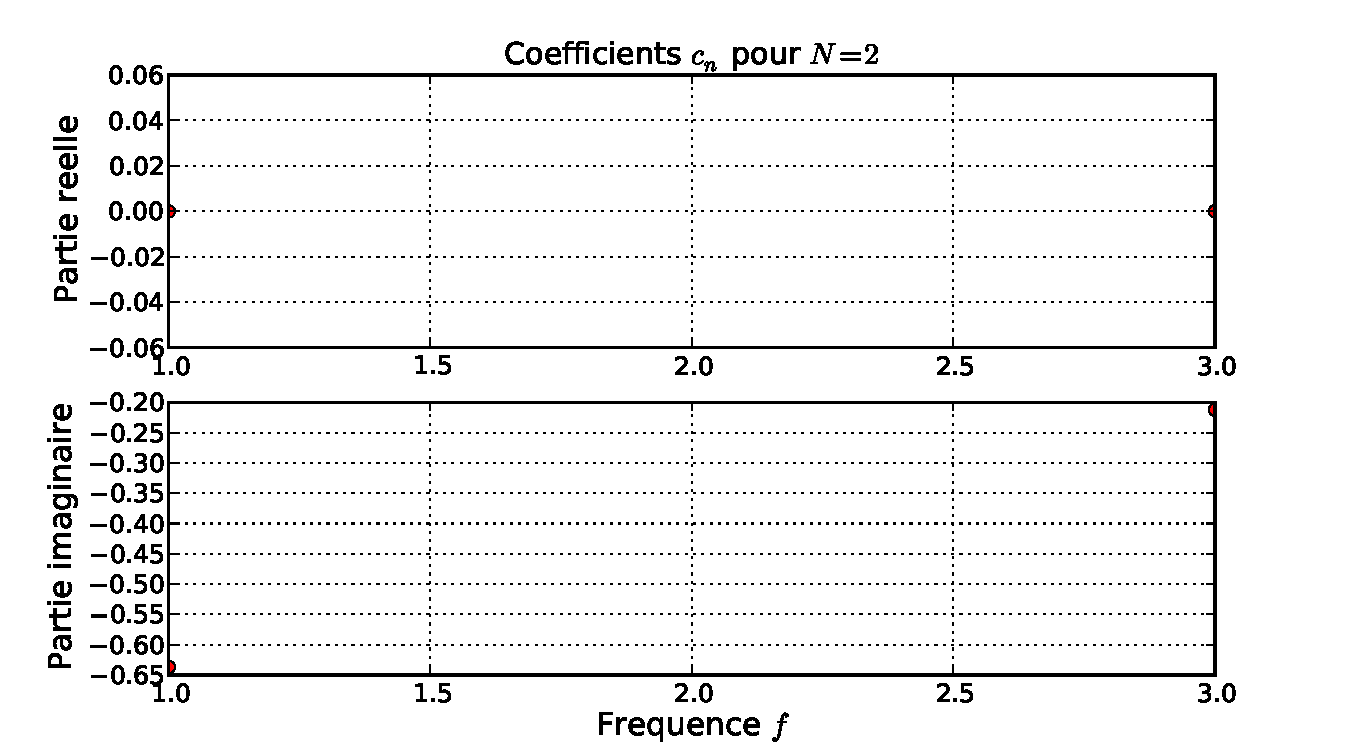
\includegraphics[width=1.\textwidth]{figures/serieF_carre_c_2.pdf} \\
\end{frame}

\begin{frame}{Exercice: signal carré}
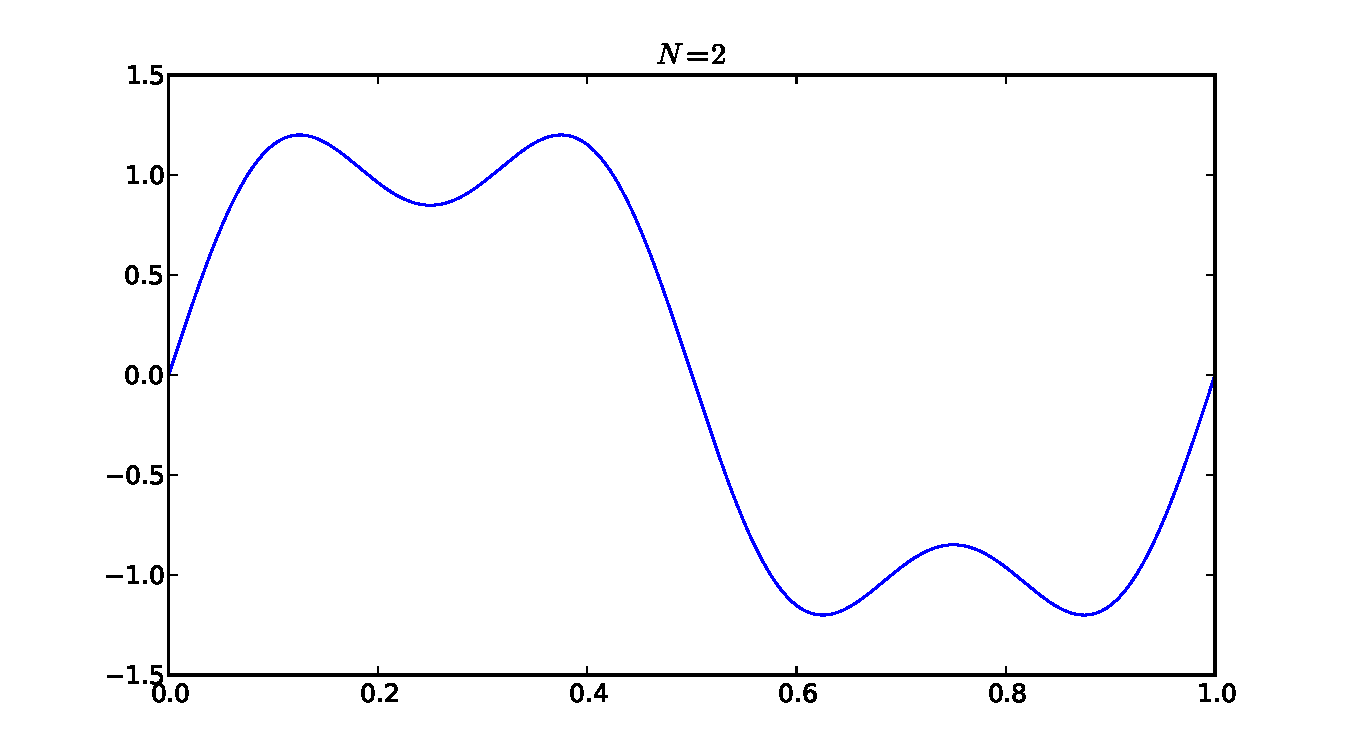
\includegraphics[width=1.\textwidth]{figures/serieF_carre_2.pdf}\\
\end{frame}

\begin{frame}{Exercice: signal carré}
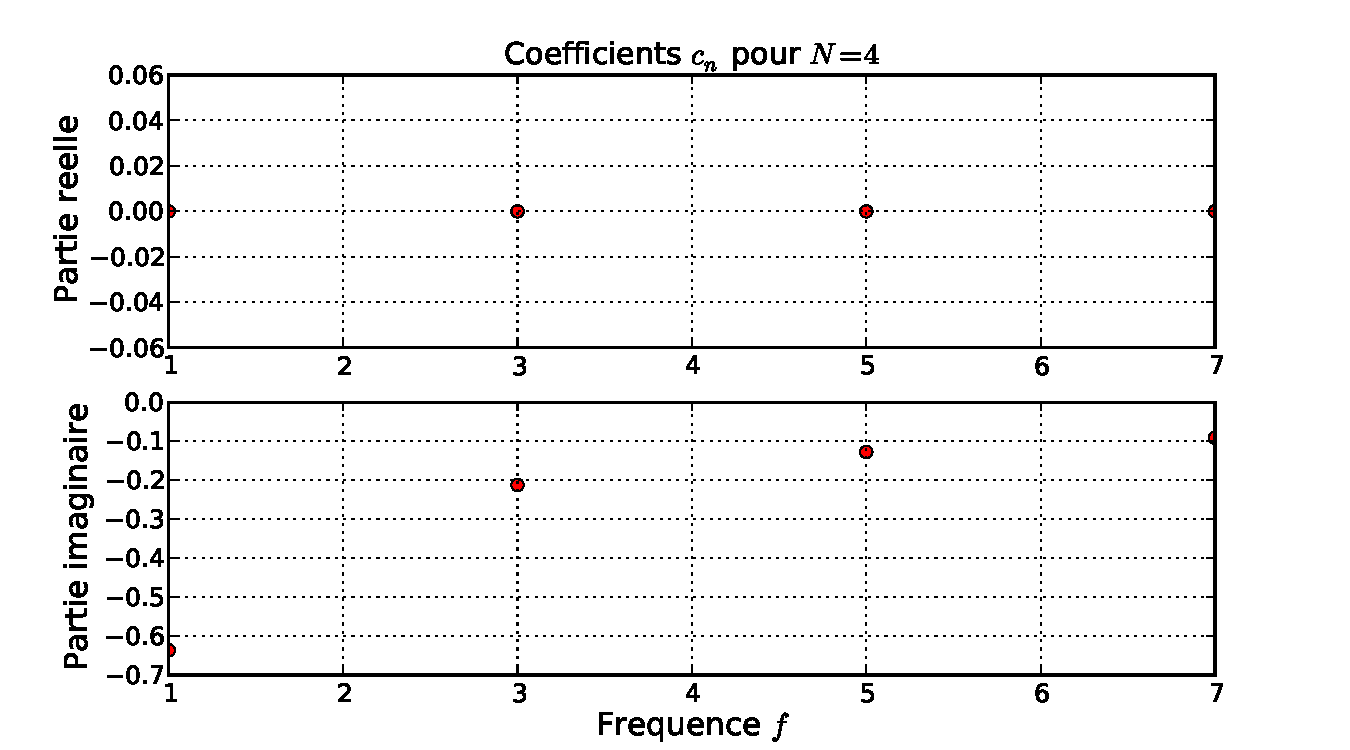
\includegraphics[width=1.\textwidth]{figures/serieF_carre_c_4.pdf} \\
\end{frame}

\begin{frame}{Exercice: signal carré}
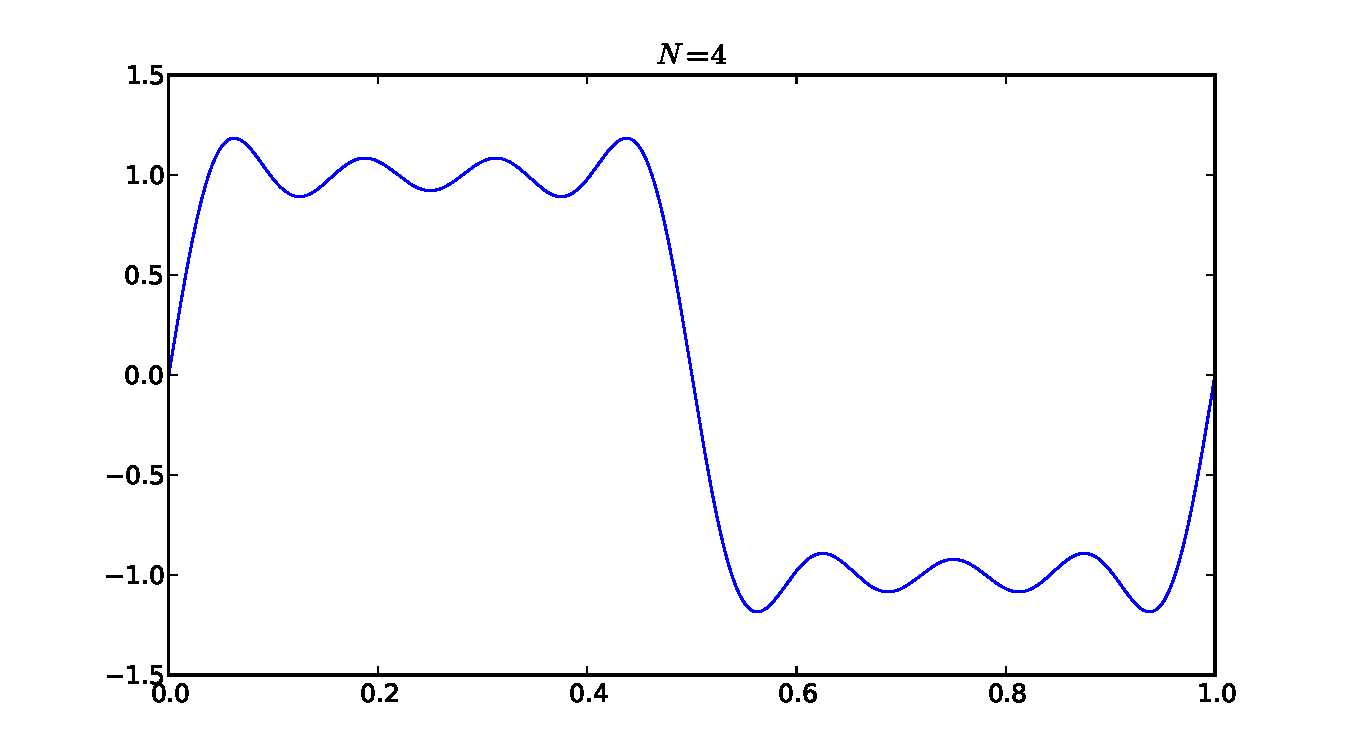
\includegraphics[width=1.\textwidth]{figures/serieF_carre_4.pdf}\\
\end{frame}


\begin{frame}{Exercice: signal carré}
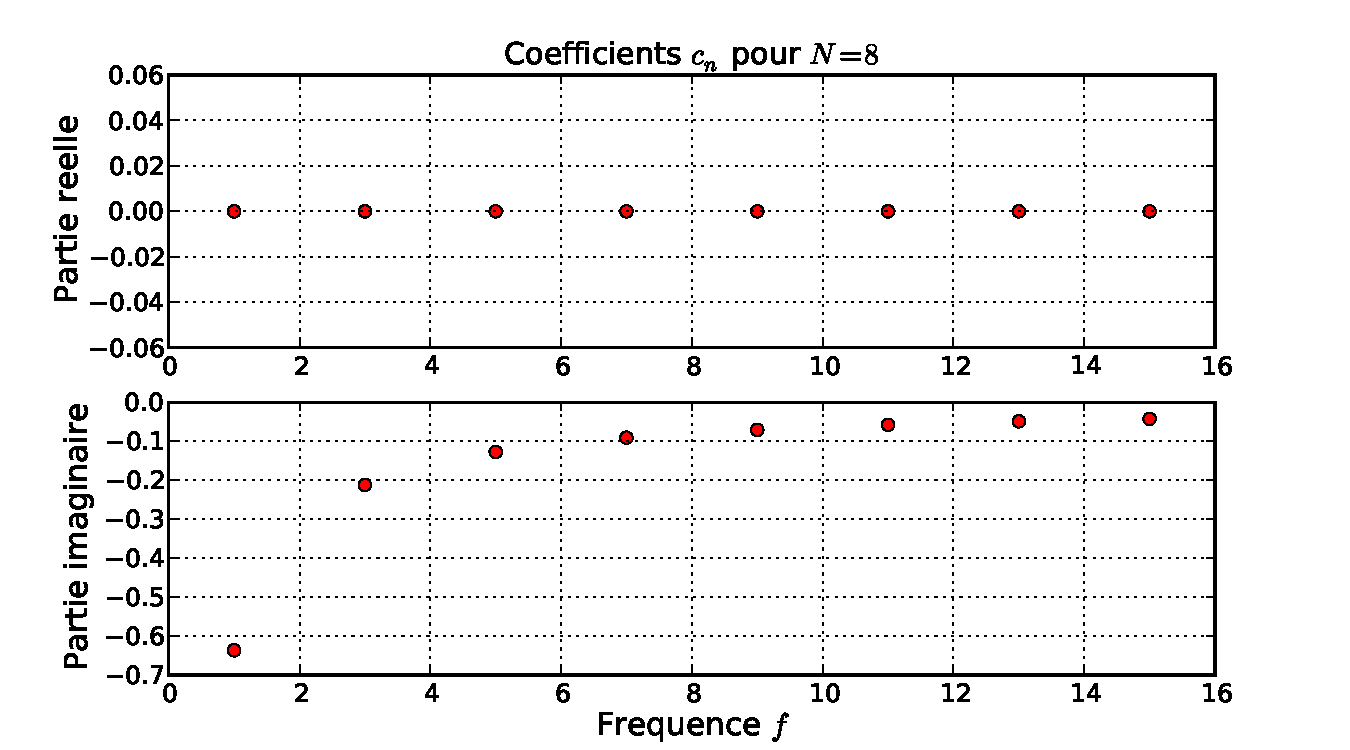
\includegraphics[width=1.\textwidth]{figures/serieF_carre_c_8.pdf} \\
\end{frame}

\begin{frame}{Exercice: signal carré}
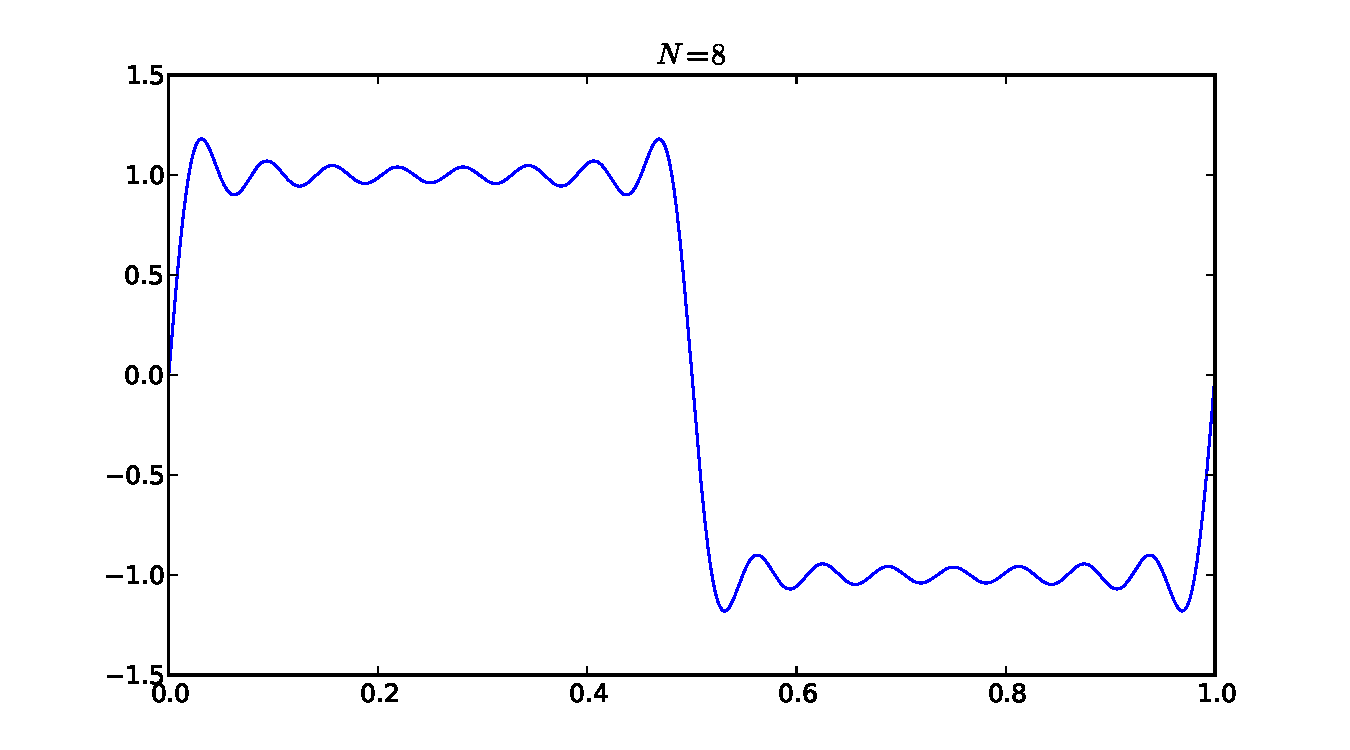
\includegraphics[width=1.\textwidth]{figures/serieF_carre_8.pdf}\\
\end{frame}

\begin{frame}{Exercice: signal carré}
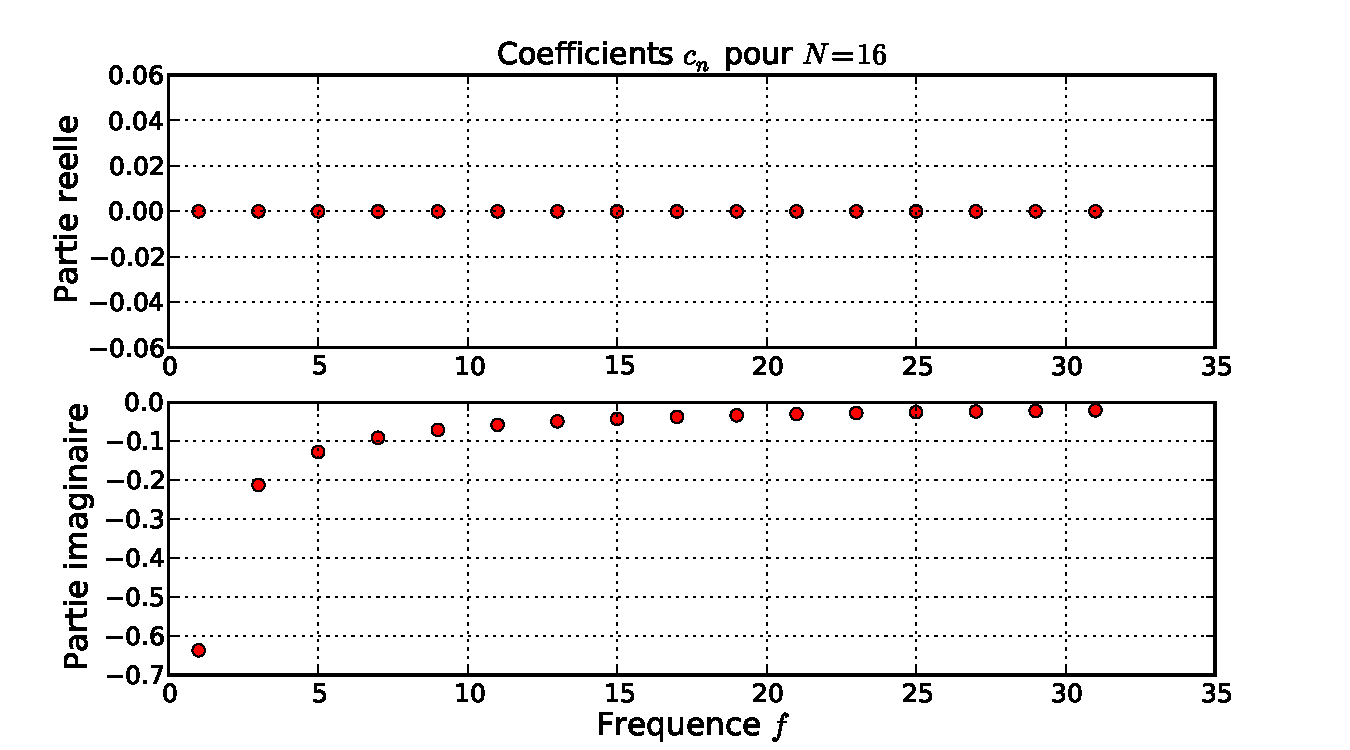
\includegraphics[width=1.\textwidth]{figures/serieF_carre_c_16.pdf} \\
\end{frame}

\begin{frame}{Exercice: signal carré}
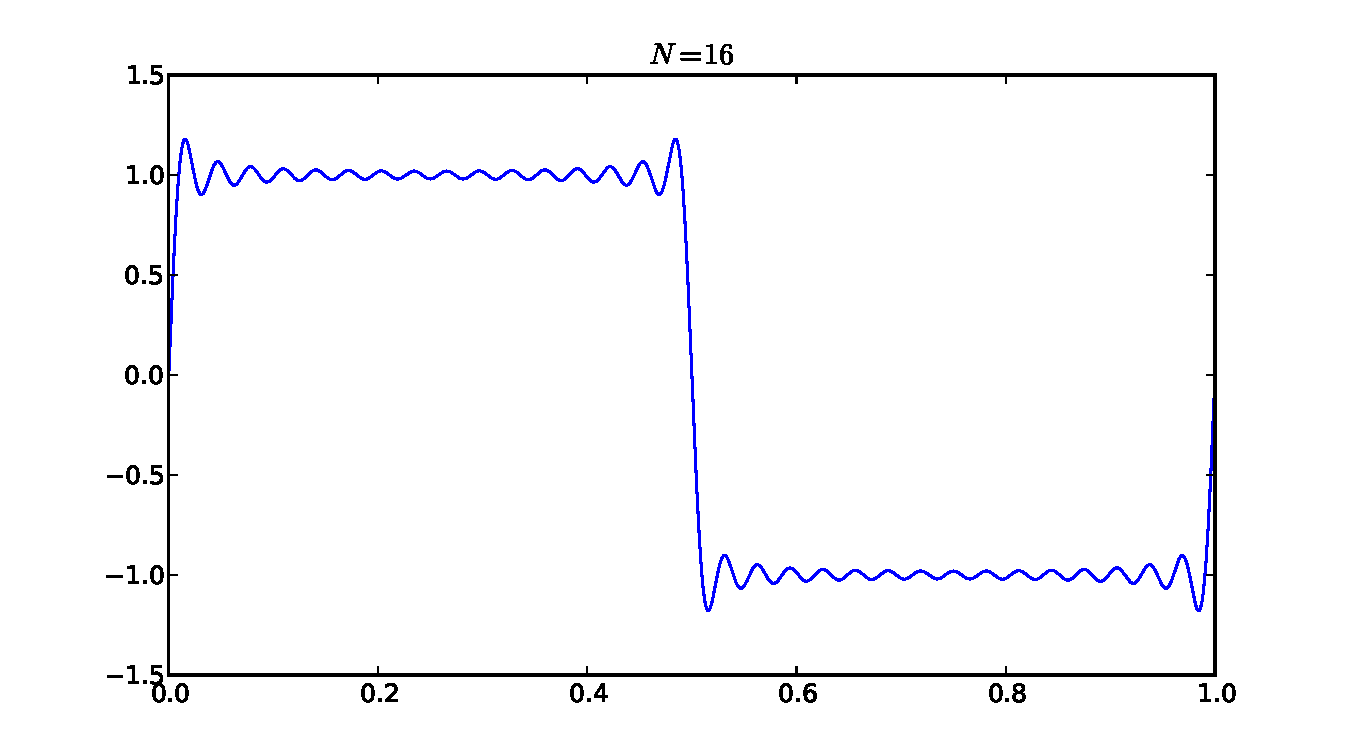
\includegraphics[width=1.\textwidth]{figures/serieF_carre_16.pdf}\\
\end{frame}

\begin{frame}{Exercice: signal carré}
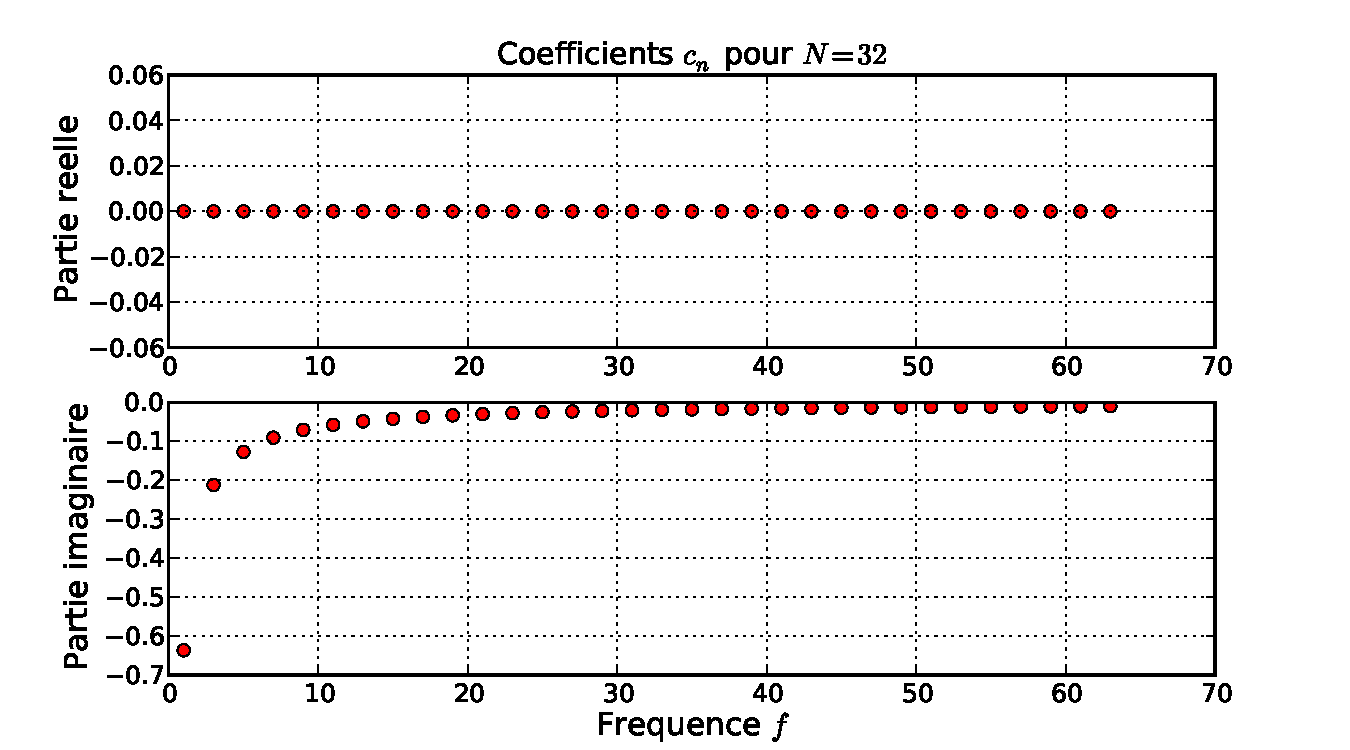
\includegraphics[width=1.\textwidth]{figures/serieF_carre_c_32.pdf} \\
\end{frame}

\begin{frame}{Exercice: signal carré}
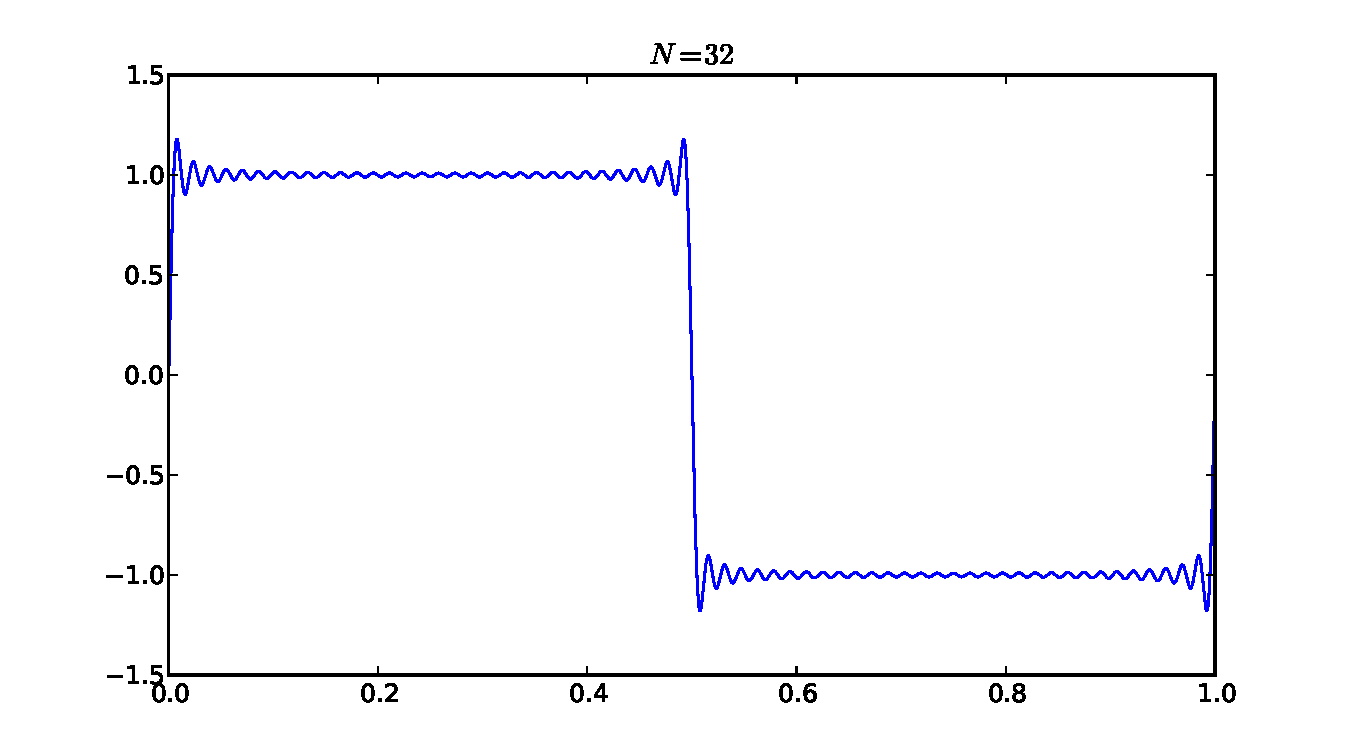
\includegraphics[width=1.\textwidth]{figures/serieF_carre_32.pdf}\\
\end{frame}

\begin{frame}{Exercice: signal carré}
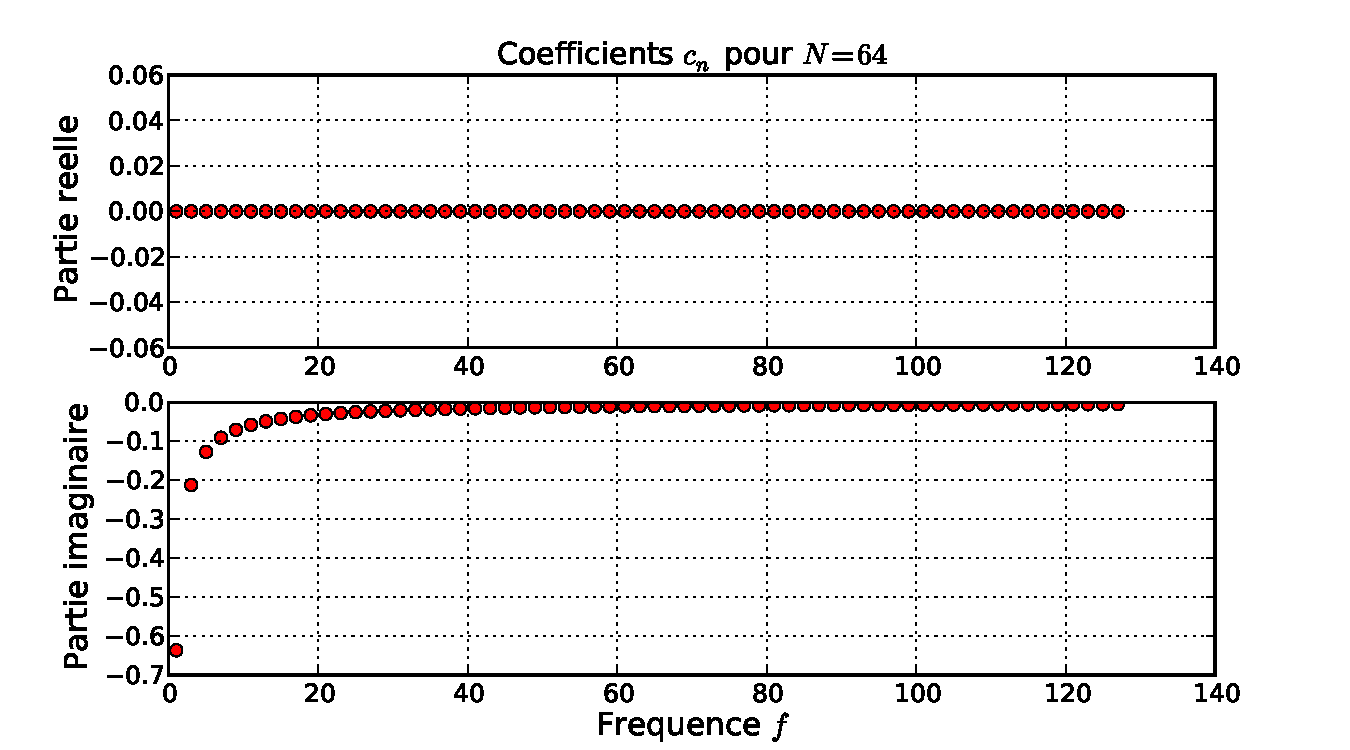
\includegraphics[width=1.\textwidth]{figures/serieF_carre_c_64.pdf} \\
\end{frame}

\begin{frame}{Exercice: signal carré}
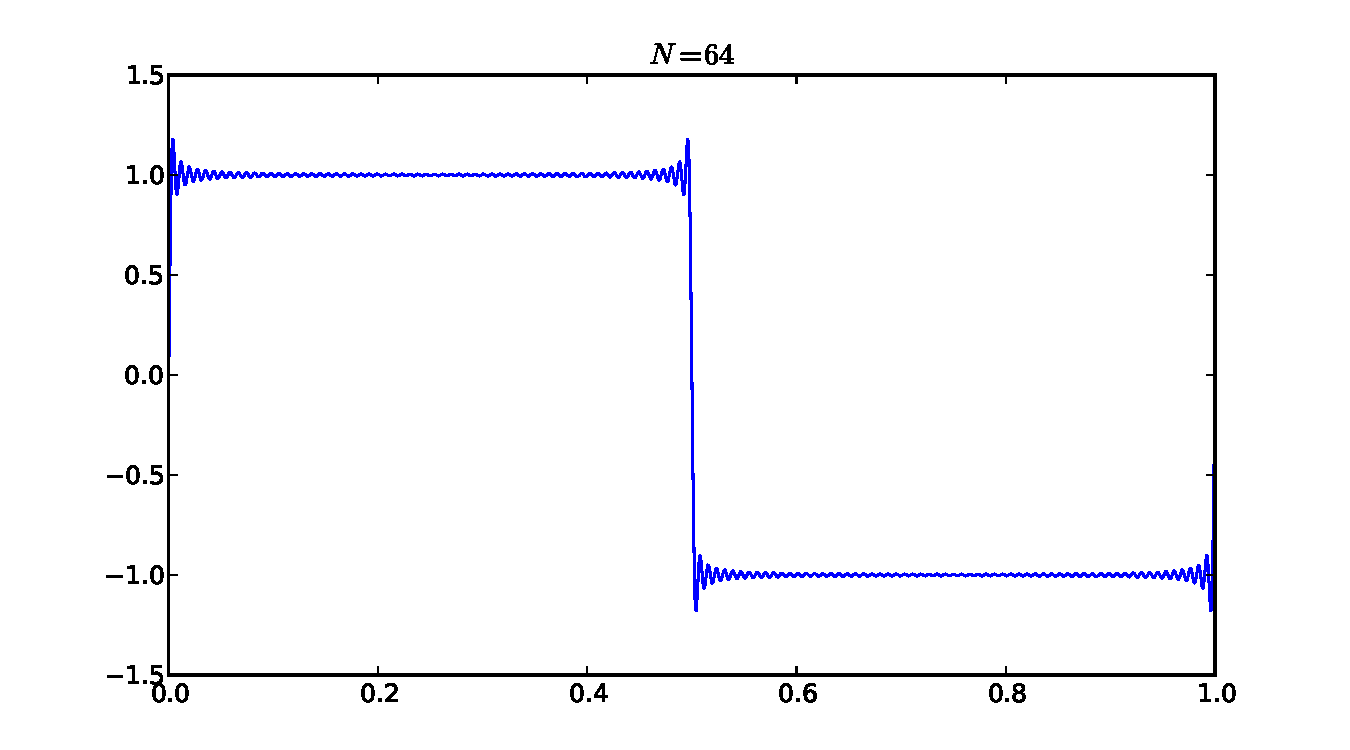
\includegraphics[width=1.\textwidth]{figures/serieF_carre_64.pdf}\\
\end{frame}

\begin{frame}{Exercice: signal carré}
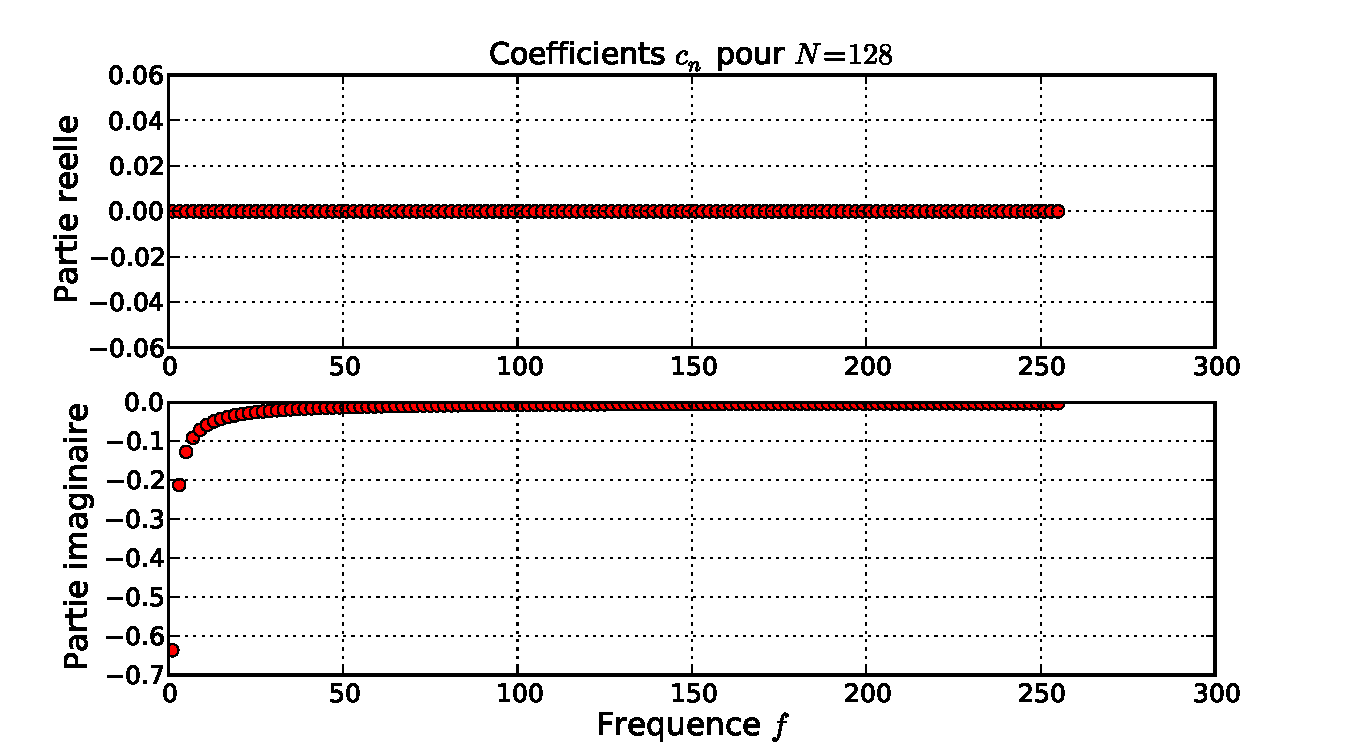
\includegraphics[width=1.\textwidth]{figures/serieF_carre_c_128.pdf} \\
\end{frame}

\begin{frame}{Exercice: signal carré}
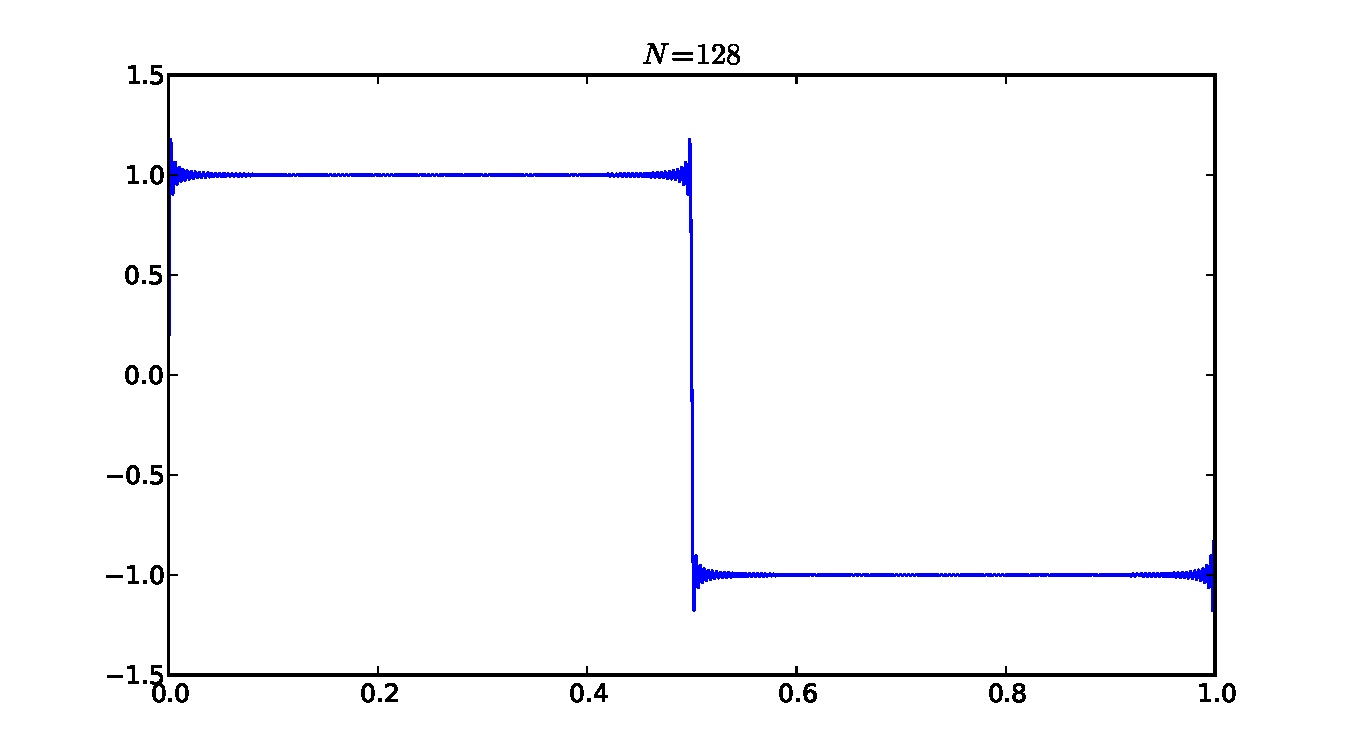
\includegraphics[width=1.\textwidth]{figures/serieF_carre_128.pdf}\\
\end{frame}

\begin{frame}{Exercice: signal carré}
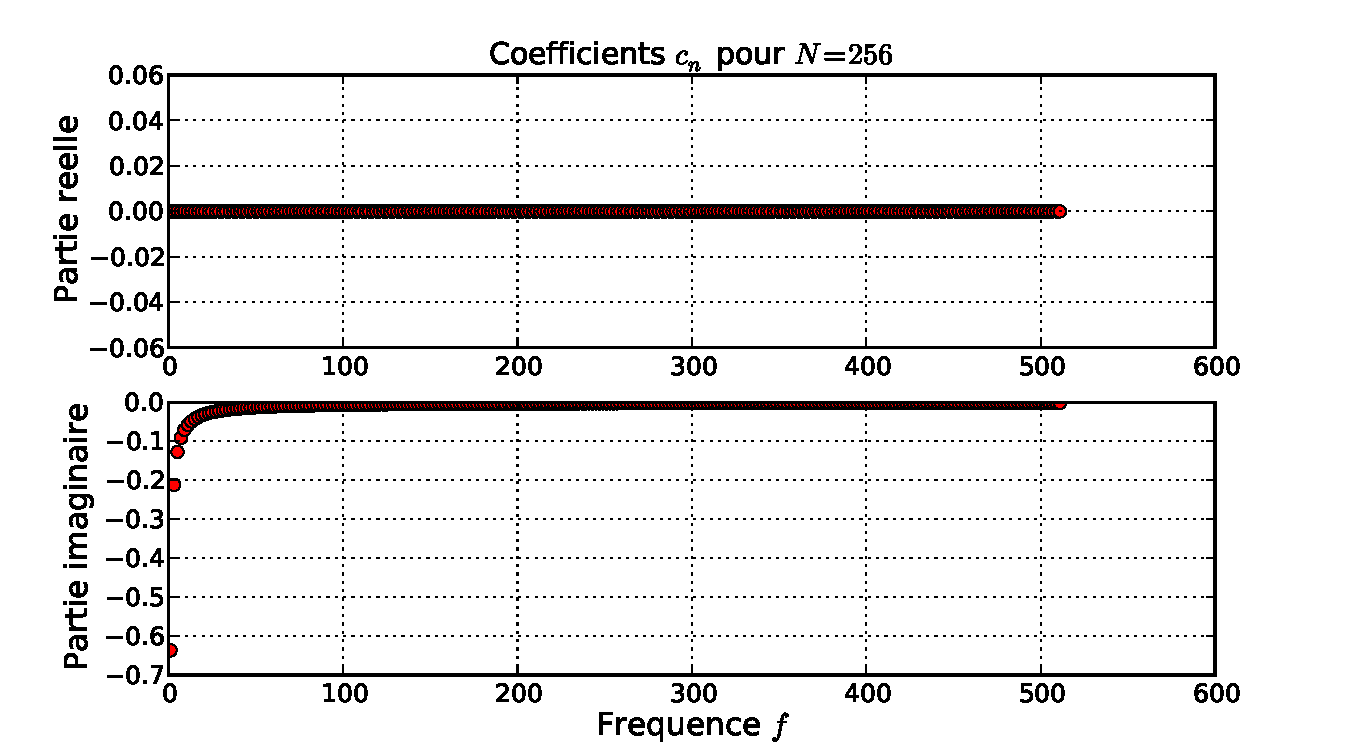
\includegraphics[width=1.\textwidth]{figures/serieF_carre_c_256.pdf} \\
\end{frame}

\begin{frame}{Exercice: signal carré}
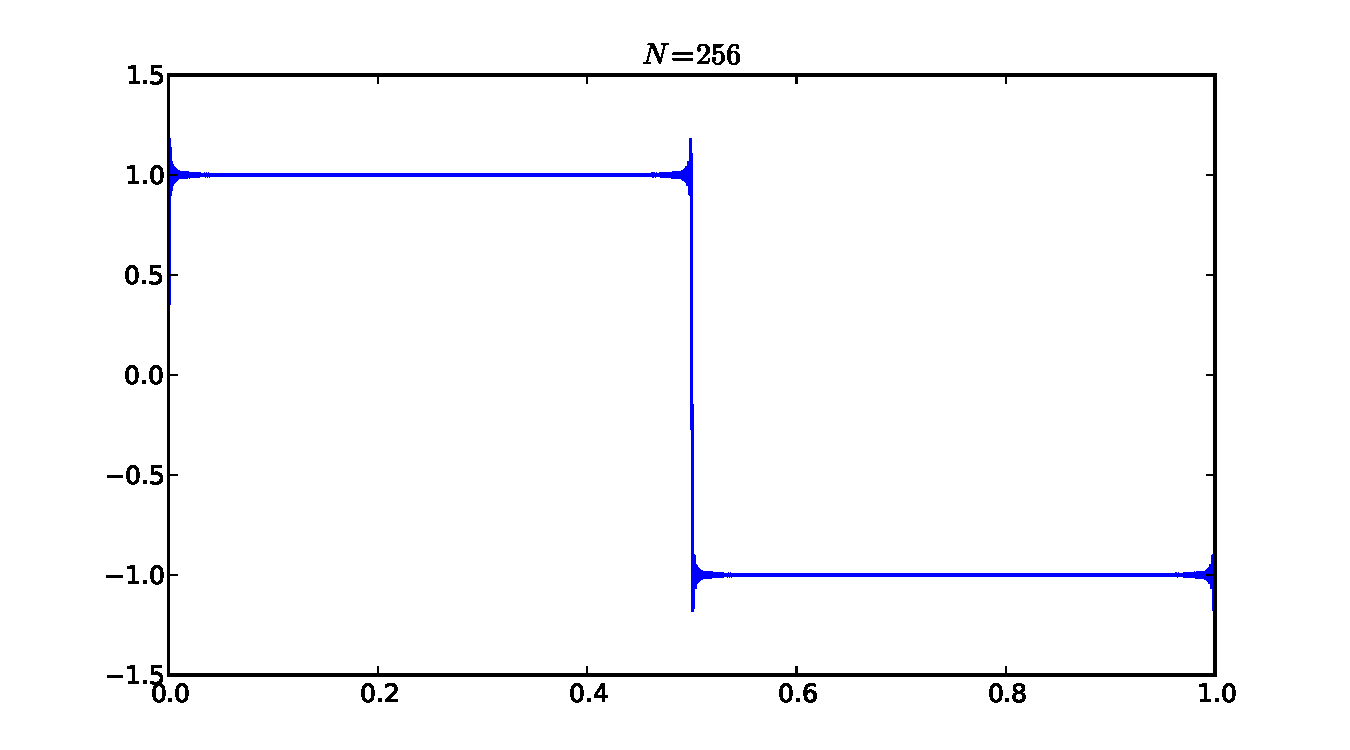
\includegraphics[width=1.\textwidth]{figures/serieF_carre_256.pdf}\\
\end{frame}

\begin{frame}{Exercice: signal carré}
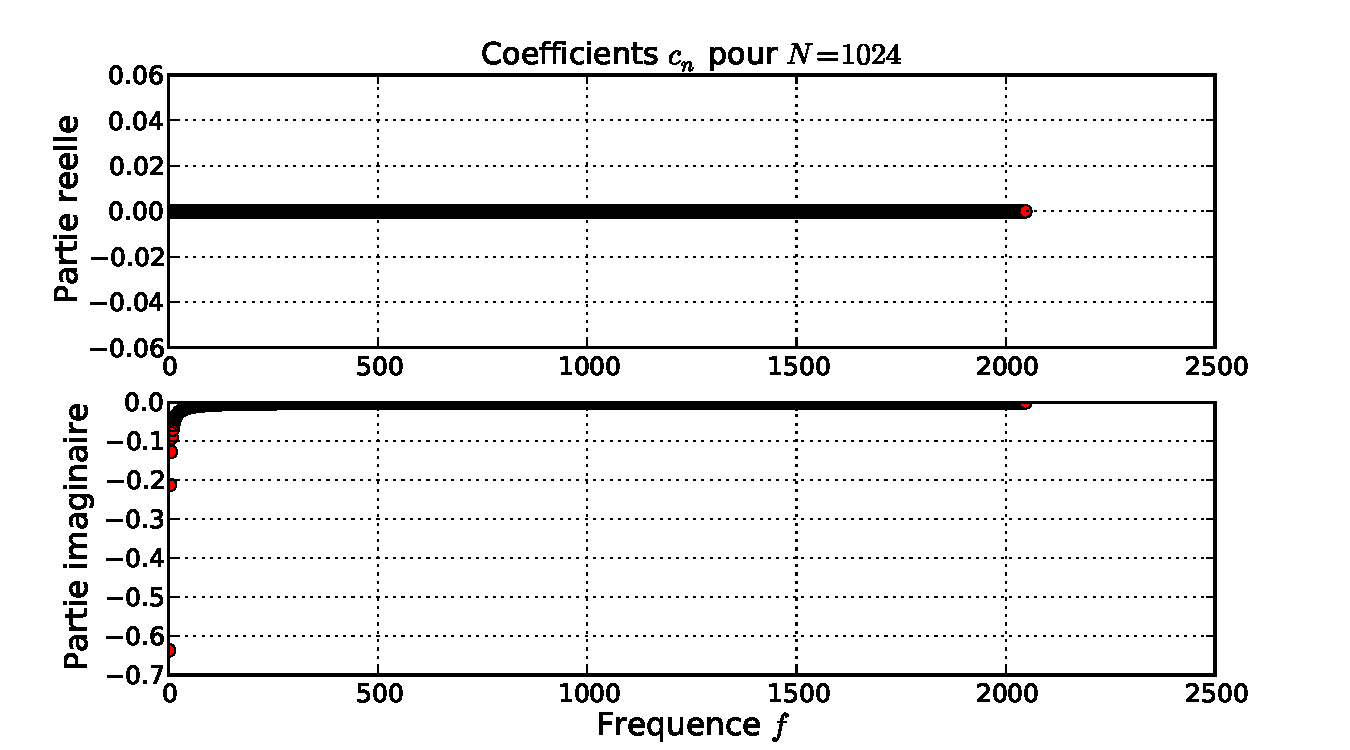
\includegraphics[width=1.\textwidth]{figures/serieF_carre_c_1024.pdf} \\
\end{frame}

\begin{frame}{Exercice: signal carré}
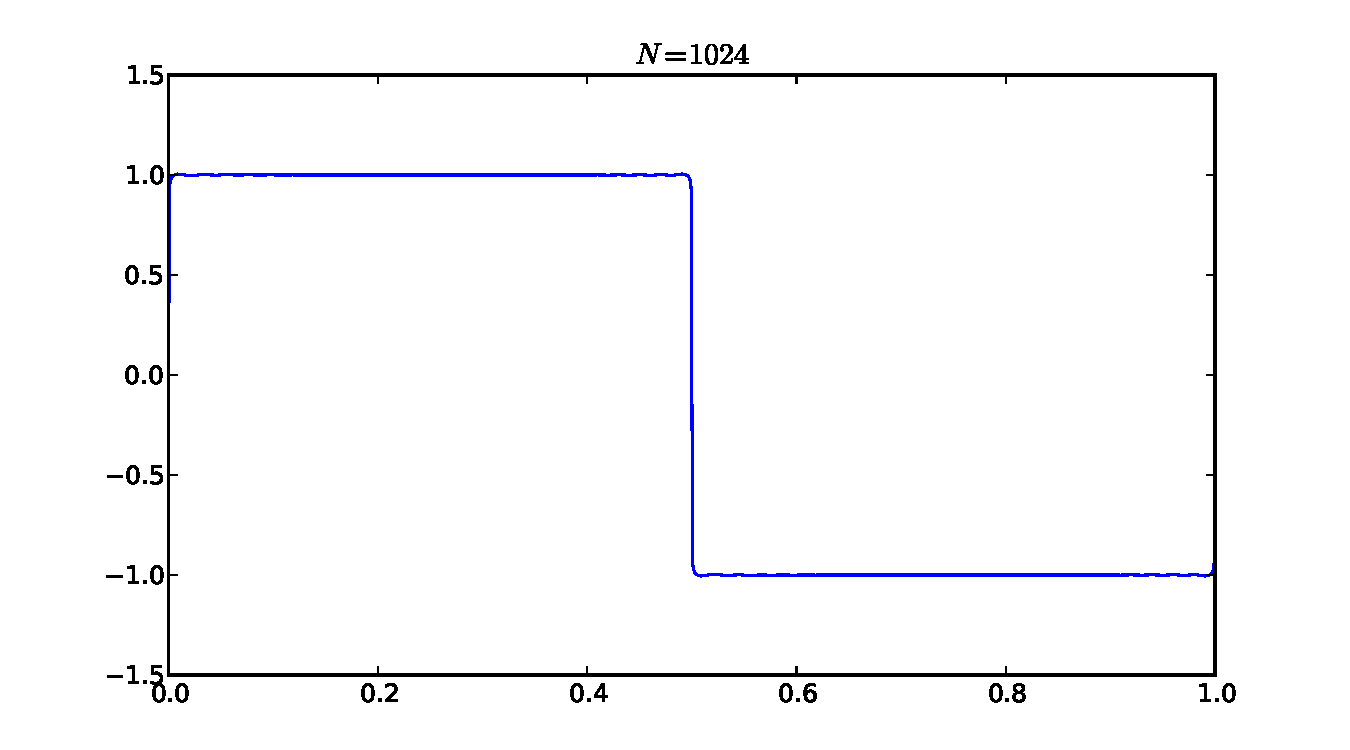
\includegraphics[width=1.\textwidth]{figures/serieF_carre_1024.pdf}\\
\end{frame}
\subsection{Extention aux signaux apériodiques}

\begin{frame}{Transformées de Fourier}



\begin{block}{Formulation}
$$
x(t) \overset{\mathcal{F}}{\longmapsto} X(f) = \int_{-\infty}^{+\infty}x(t)e^{-2j\pi ft}dt
$$
$$
X(f) \overset{\mathcal{F}^{-1}}{\longmapsto} x(t) = \int_{-\infty}^{+\infty}X(f)e^{2j\pi ft}df
$$
\end{block}

\begin{alertblock}{Points clés}
\begin{itemize}
\item $\mathcal F$ est la tranformée de Fourier et $\mathcal F^{-1}$ la transformée de Fourier inverse.
\item $\mathcal F$ s'applique à tous les signaux, même apériodiques.
\item $X(f)$ est le spectre de $x(t)$.
\item Un signal apériodique possède un spectre continu.
\item Un signal périodique possède un spectre discret. 
\end{itemize}
\end{alertblock}
\end{frame}


%\section{Traitement des signaux discrets}
  \subsection{La Transformée de Fourier Discrète (DFT)}
  \begin{frame}{La Transformée de Fourier Discrète ou DFT}
  \begin{block}{Formulation}
  On considère un signal échantilloné $[x_n]$ comportant N échantillons. Sa transformée de Fourier discrètre $[X_k]$ s'écrit:
$$ 
  [x_n] \overset{\mathcal{DFT}}{\longmapsto} [X_k] = \sum\limits_{n=0}^{n=N-1}x_n e^{-2j\pi \frac{kn}{N}}
$$
$$
[X_k] \overset{\mathcal{DFT}^{-1}}{\longmapsto} [x_n] = \frac{1}{N}\sum\limits_{k=0}^{k=N-1}X_k e^{2j\pi \frac{kn}{N}}
$$
  
  \end{block}
  \begin{block}{Interprétation de $[X_k]$ }
  Le vecteur $X_k$ représente le spectre discret de $[x_n]$. Chaque coefficient $X_k$ est associé à une fréquence $f_k$ obtenue par:
  $$
  f_k = k/D = kf_e/{N}
  $$
  \end{block}
  \end{frame}
  \subsection{La Transformée de Fourier Rapide (FFT)}
  \begin{frame}{La Transformée de Fourier Discrète ou DFT}
  \begin{block}{Interprétation de $[X_k]$ }
  Dans le cas ou le signal $x(t)$ est réel, les coefficients $X_k$ pour $k>N/2$ sont les conjugués des coefficients d'indice $k<N/2$. On peut donc se contenter d'interprêter les $N/2$ premiers coefficients. 
  \end{block}
  \begin{block}{Liens entre $[X_k]$ et $[a_k,b_k]$ }
  Les coefficients $a_k$ et $b_k$ peuvent \^etre déterminés par:
  \begin{align}
  a_k & = \frac{2}{N} \Re(X_k)\nonumber \\  
  b_k & = -\frac{2}{N} \Im(X_k)\nonumber
  \end{align}
  \end{block}
  \end{frame}
  \begin{frame}[containsverbatim]
  \frametitle{Mise en pratique: calcul de la DFT}
\begin{block}{Programme de calcul de la DFT}
\lstinputlisting{listings/exemple_DFT.py}
\end{block}
\end{frame}

\begin{frame}{Vérification la DFT sur un signal sinusoïdal}
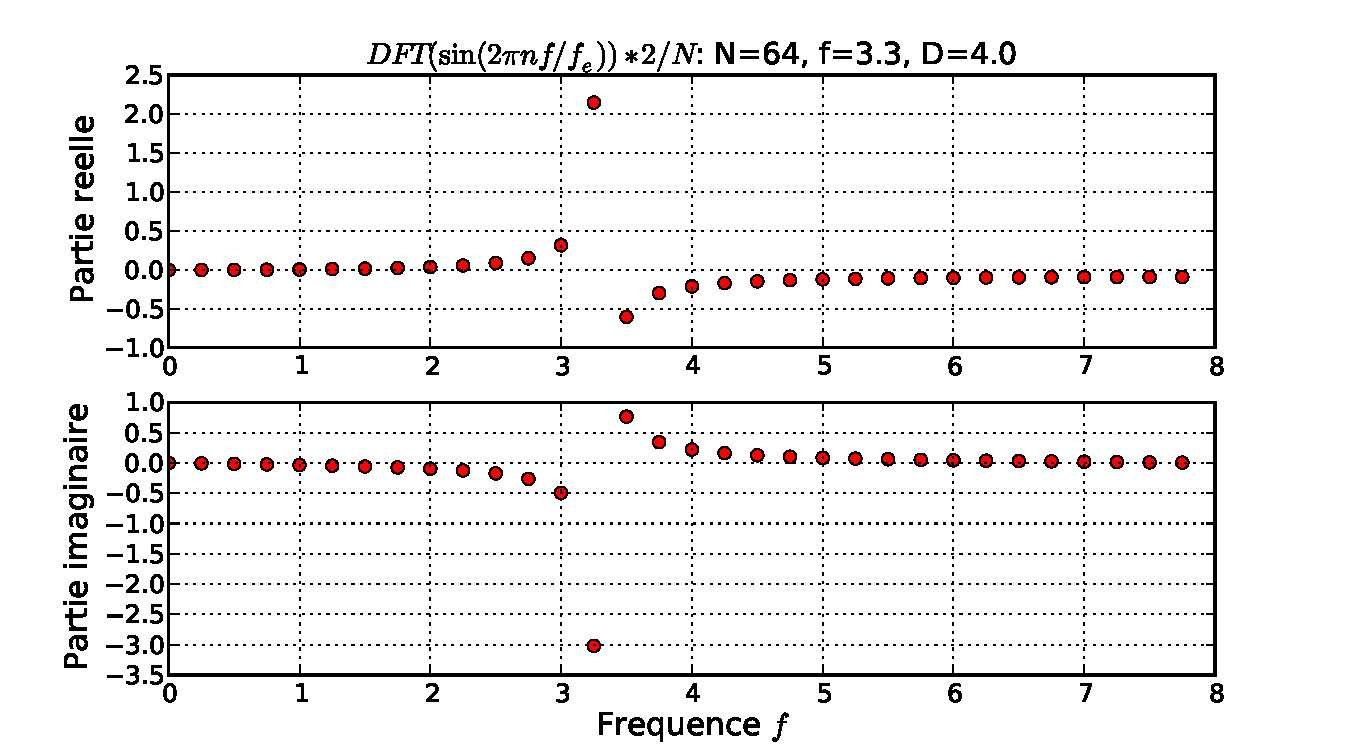
\includegraphics[width=1.\textwidth]{figures/DFT_sinus.pdf} \\
On retrouve donc bien la série de Fourier avec le coefficient $2/N$.
\end{frame}

\subsection{Optimisation de la DFT: la Transformée de Fourier Rapide (FFT)}

\begin{frame}{La FFT, pourquoi ? Comment ?}
\begin{block}{Pourquoi ?}
\begin{itemize}
\item Le calcul direct de la DFT demande de l'ordre de $N^2$ opérations alors que des algorithmes optimisés dits FFT demandent $N\times\log N$ opérations. Le gain de temps est très significatif quand $N$ est grand.
\item L'utilisation de langages rapides (C, Fortran) dans le module FFTPack disponible dans Scipy permet typiquement d'augmenter d'un facteur 400 la vitesse d'execution par rapport Python.
\end{itemize}
\end{block}

\begin{block}{Comment ?}
\begin{itemize}
\item Restrictions de la FFT: $N$ doit être une puissance de 2.
\item Utilisation:
\lstinputlisting{listings/exemple_FFT.py}
Renvoie $X_n = [0,-2j,0,2j]$ ce qui est identique au résultat obtenu par DFT. On utilisera donc préférentiellement la FFT pour des raisons de commodité et vitesse.
\end{itemize}
\end{block}
\end{frame}

\begin{frame}{FFT: effet de la fréquence $f$}
\begin{block}{Programme}
\lstinputlisting[lastline=28]{listings/exemple_FFT_frequence.py}
\end{block}
\end{frame}
\begin{frame}{FFT: effet de la fréquence $f$}
\begin{block}{Programme}
\lstinputlisting[firstline=29,firstnumber=29]{listings/exemple_FFT_frequence.py}
\end{block}
\end{frame}

\begin{frame}{FFT: effet de la fréquence $f$}
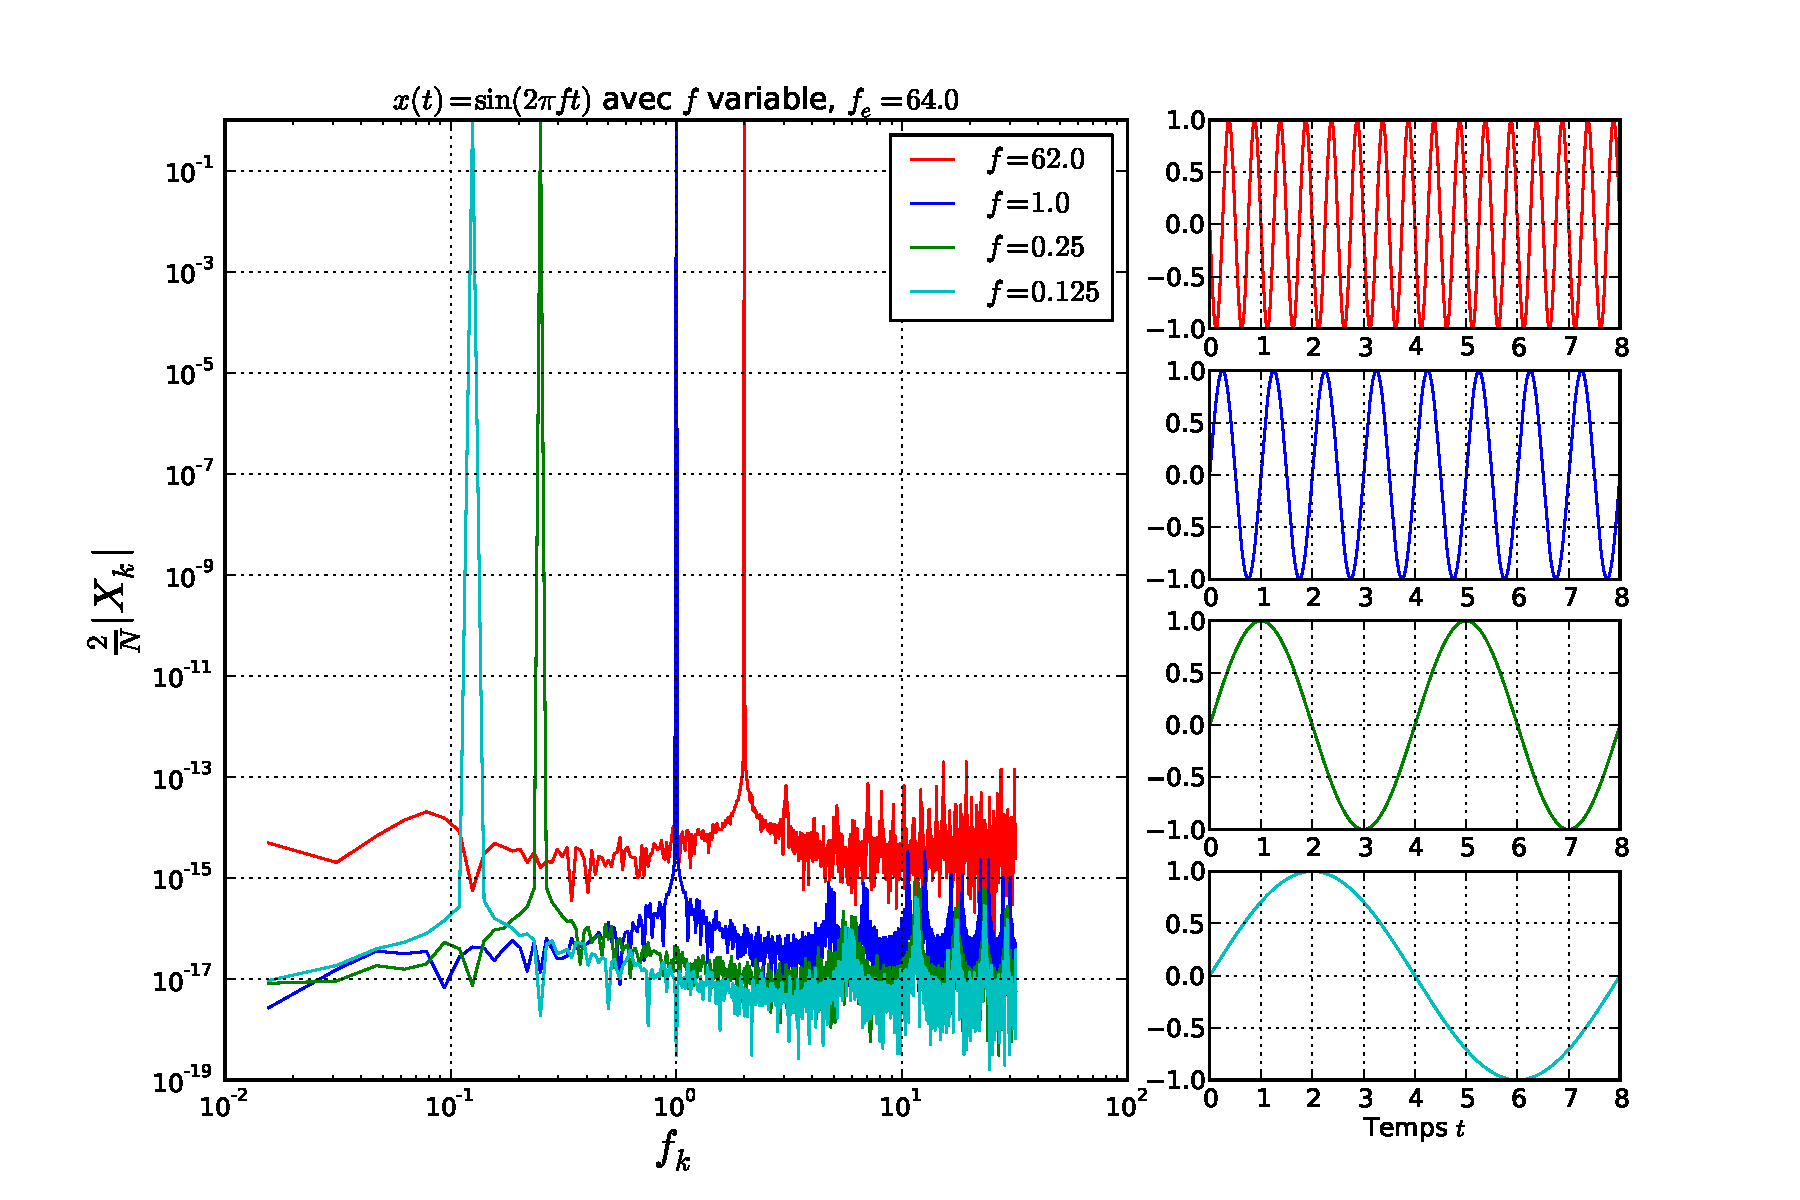
\includegraphics[width=1.\textwidth]{figures/FFT_frequence.pdf} \\
\alert{Changer la fréquence, c'est translater horizontalement le pic.}
\end{frame}



\begin{frame}{FFT: effet de la durée d'observation $D$}
\begin{block}{Programme}
\lstinputlisting[lastline=28]{listings/exemple_FFT_D.py}
\end{block}
\end{frame}
\begin{frame}{FFT: effet de la durée d'observation $D$}
\begin{block}{Programme}
\lstinputlisting[firstline=29,firstnumber=29]{listings/exemple_FFT_D.py}
\end{block}
\end{frame}

\begin{frame}{FFT: effet de la durée d'observation $D$}
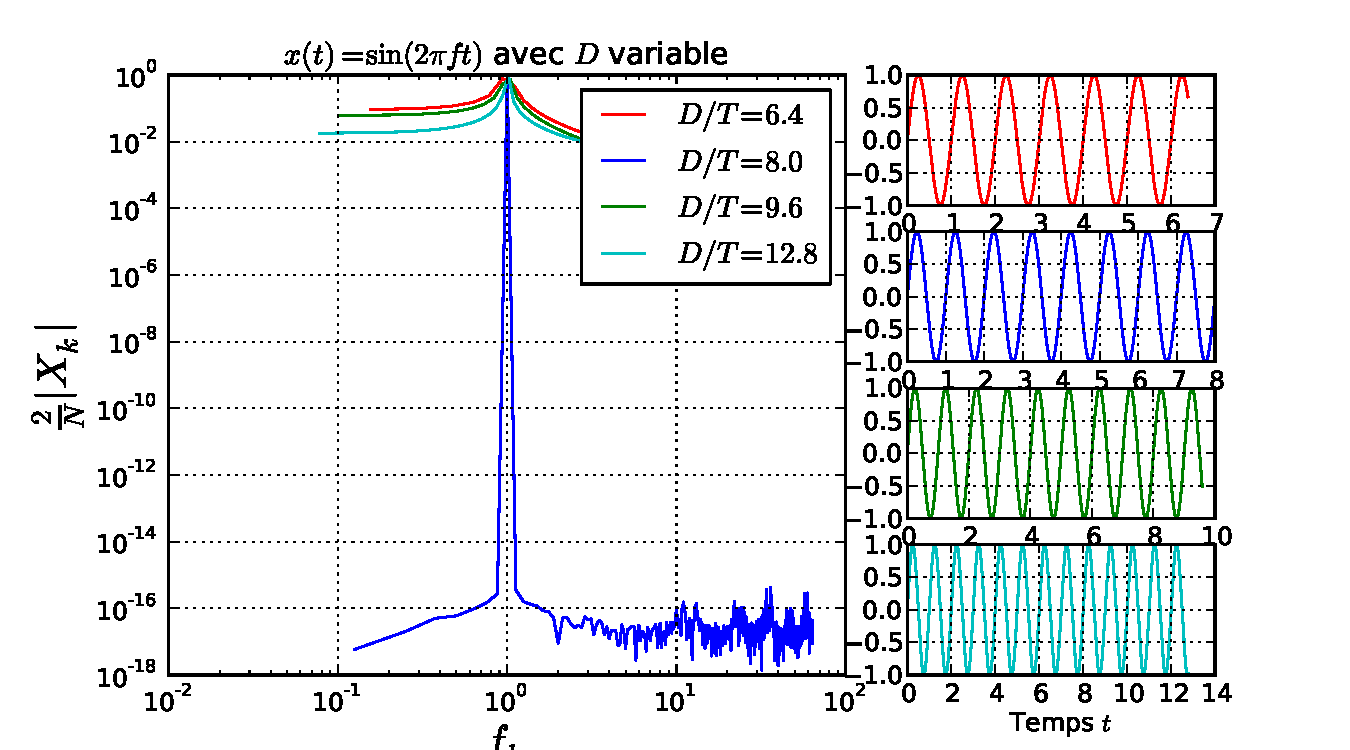
\includegraphics[width=1.\textwidth]{figures/FFT_D.pdf} \\
\alert{Lorque $D$ n'est pas multiple de la période $T$, la hauteur du pic est réduite.}
\end{frame}

\begin{frame}{FFT: effet de la durée d'observation $D$}
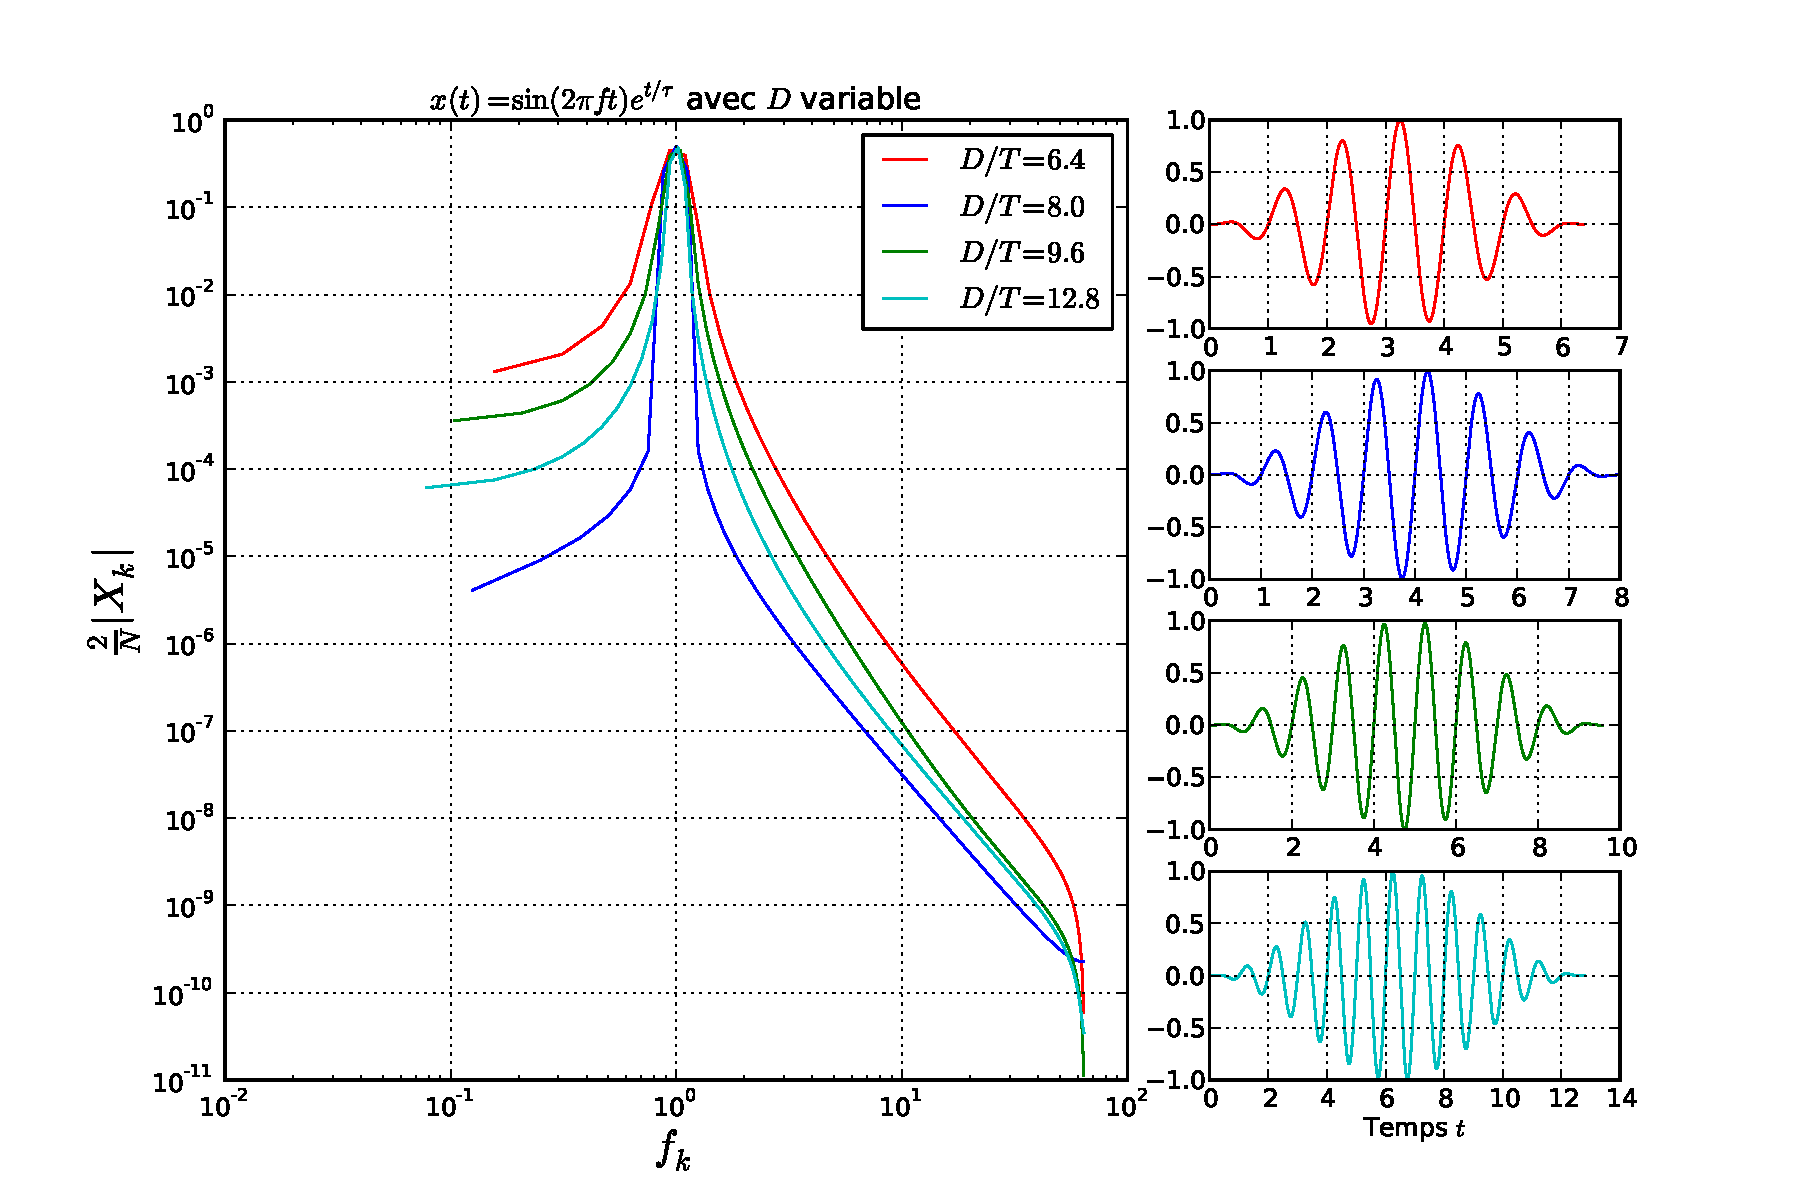
\includegraphics[width=1.\textwidth]{figures/FFT_D-hann.pdf} \\
\alert{Le fenetrage temporel de Hann permet d'augmenter la hauteur du pic.}
\end{frame}


\begin{frame}{FFT: effet du bruit}
\begin{block}{Programme}
\lstinputlisting[lastline=28]{listings/exemple_FFT_bruit.py}
\end{block}
\end{frame}
\begin{frame}{FFT: effet du bruit}
\begin{block}{Programme}
\lstinputlisting[firstline=29,firstnumber=29]{listings/exemple_FFT_bruit.py}
\end{block}
\end{frame}

\begin{frame}{FFT: effet du bruit}
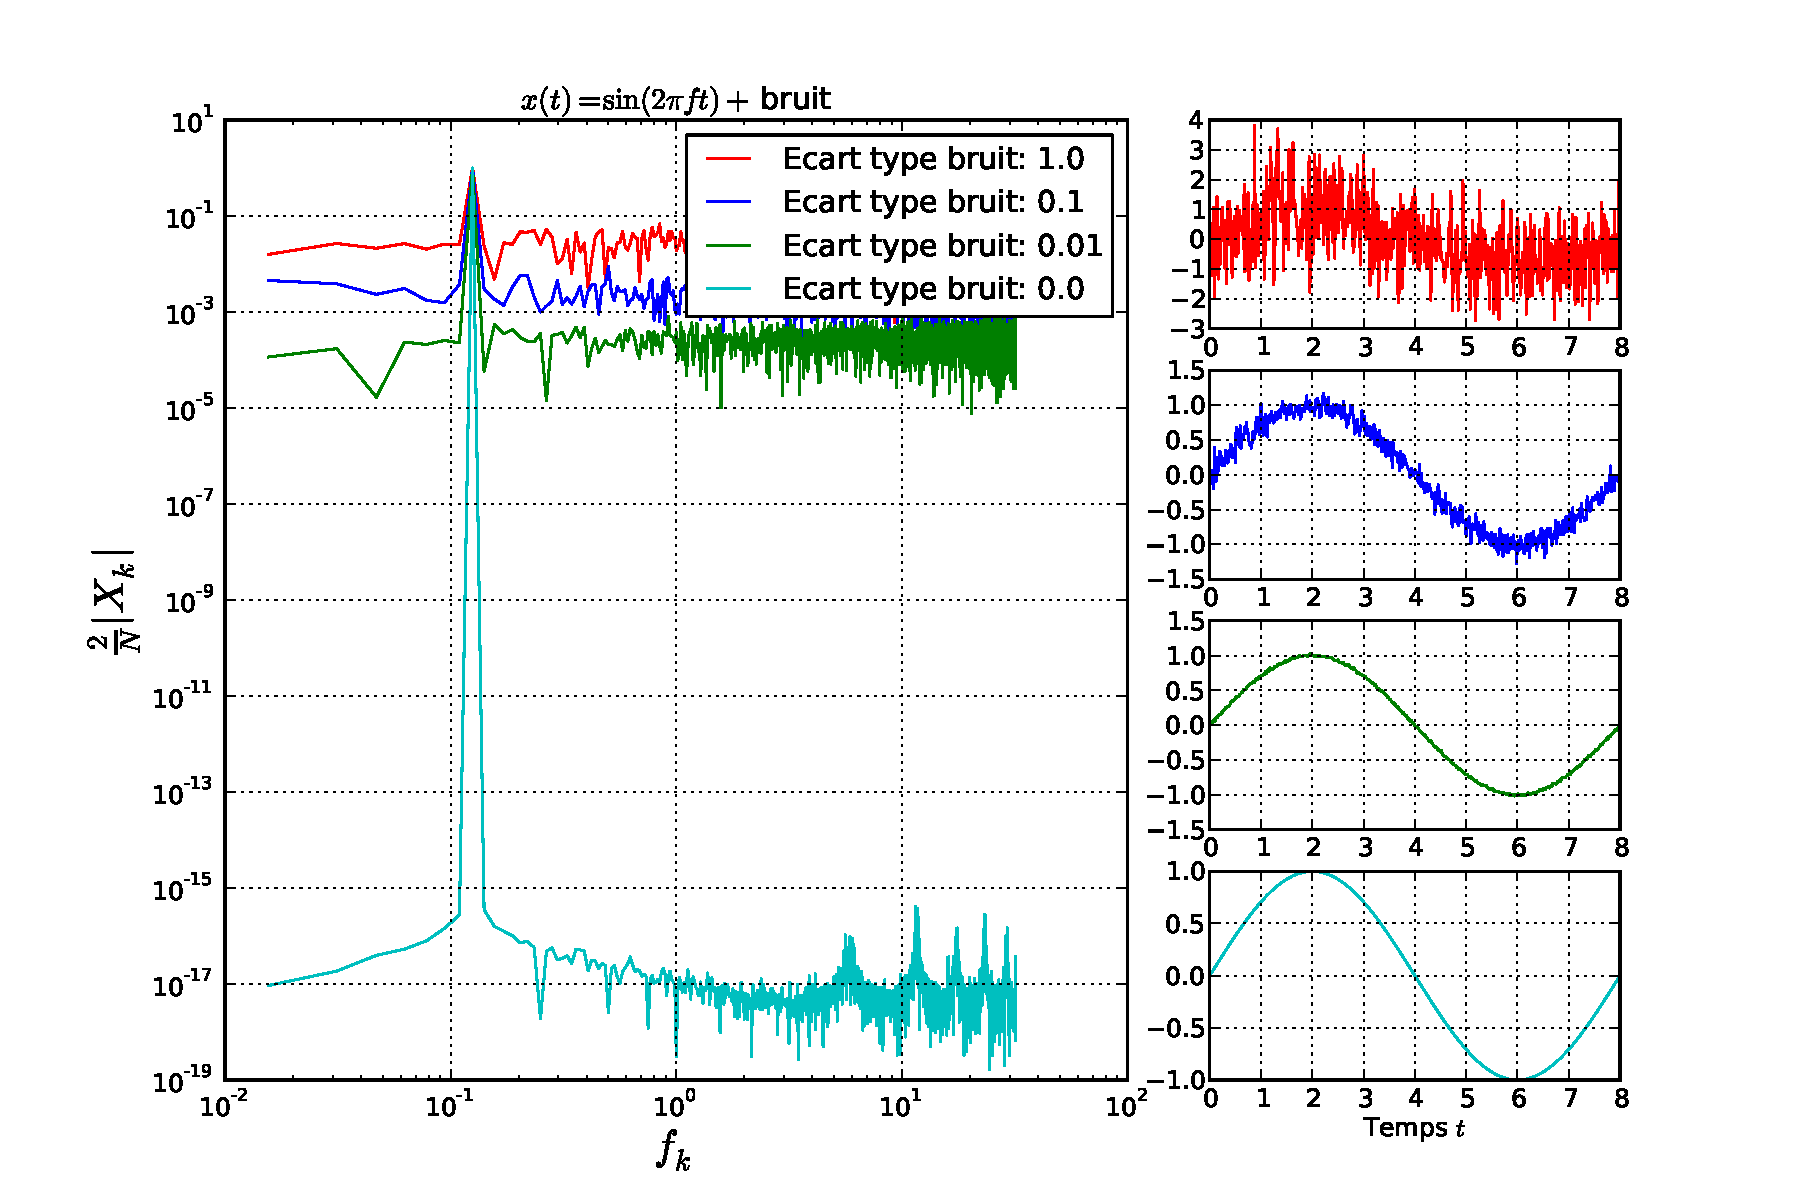
\includegraphics[width=1.\textwidth]{figures/FFT_bruit.pdf} \\
\alert{Le bruit réduit la hauteur du pic.}
\end{frame}



\begin{frame}{FFT: effet de l'amortissement}
\begin{block}{Programme}
\lstinputlisting[lastline=28]{listings/exemple_FFT_amortissement.py}
\end{block}
\end{frame}
\begin{frame}{FFT: effet de l'amortissement}
\begin{block}{Programme}
\lstinputlisting[firstline=29,firstnumber=29]{listings/exemple_FFT_amortissement.py}
\end{block}
\end{frame}

\begin{frame}{FFT: effet de l'amortissement}
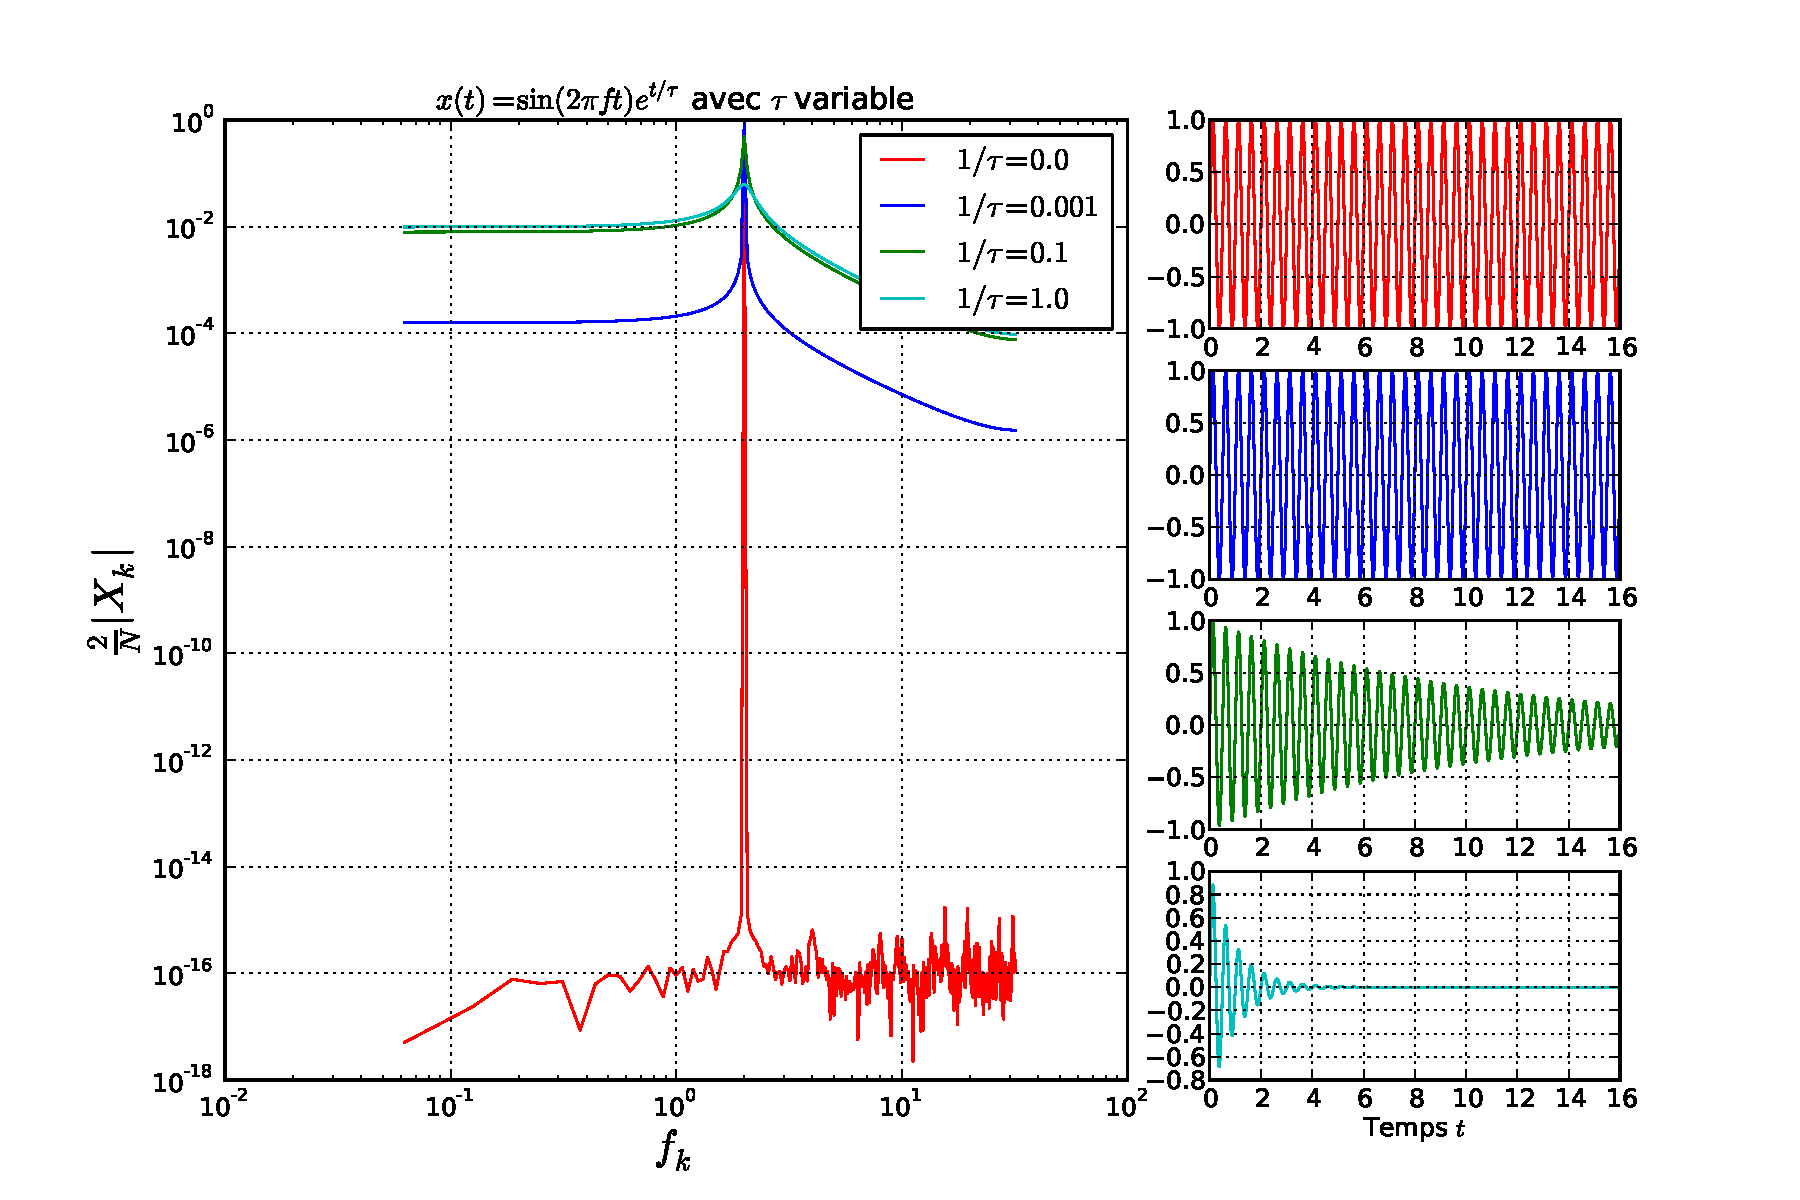
\includegraphics[width=1.\textwidth]{figures/FFT_amortissement.pdf} \\
\alert{L'amortissement entraine une perte de hauteur du pic.}
\end{frame}

\begin{frame}{FFT: amortissement et fenetrage de Hann}
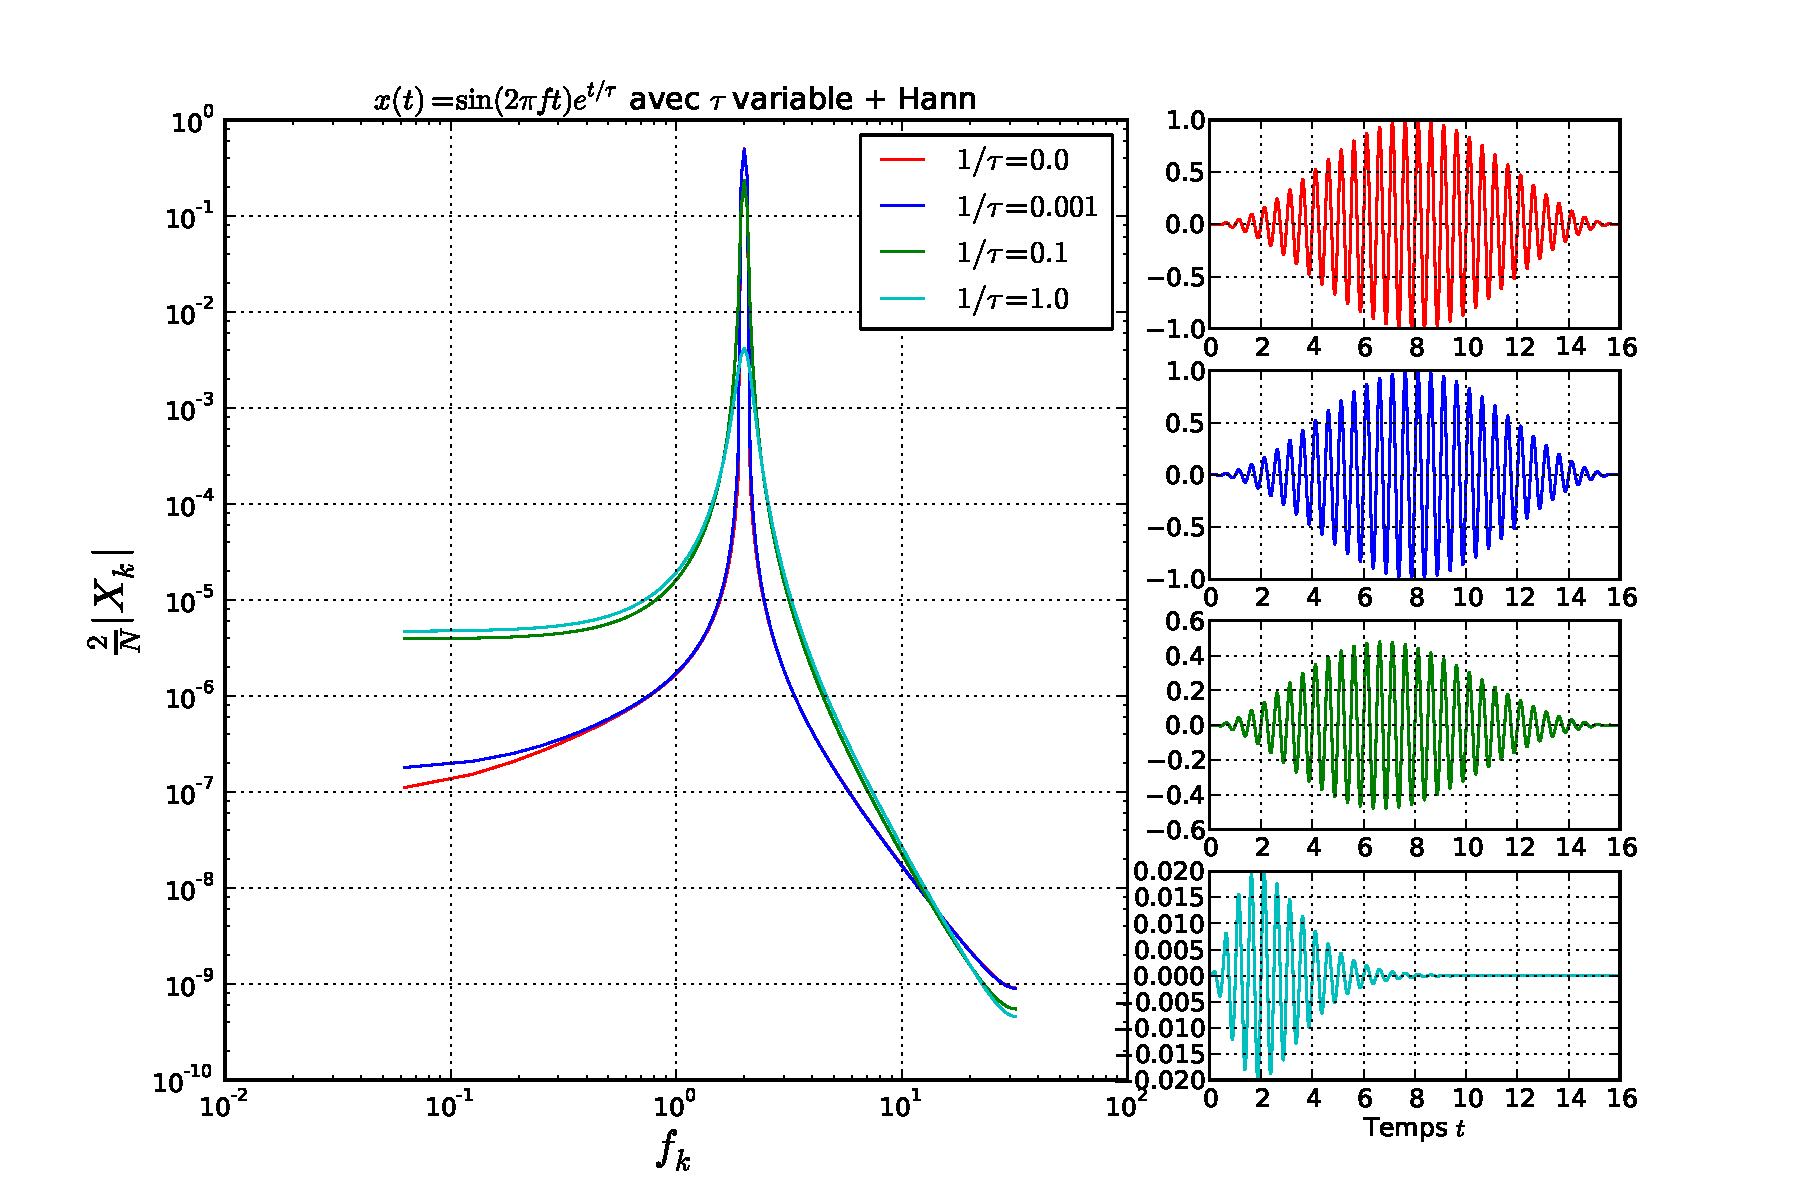
\includegraphics[width=1.\textwidth]{figures/FFT_amortissement-hann.pdf} \\
\alert{Le fenêtrage de Hann (méthode dite hanning) induit une hauteur de pic $\times 1000$ !!}
\end{frame}

\begin{frame}{Vibration d'une poutre: spectre}
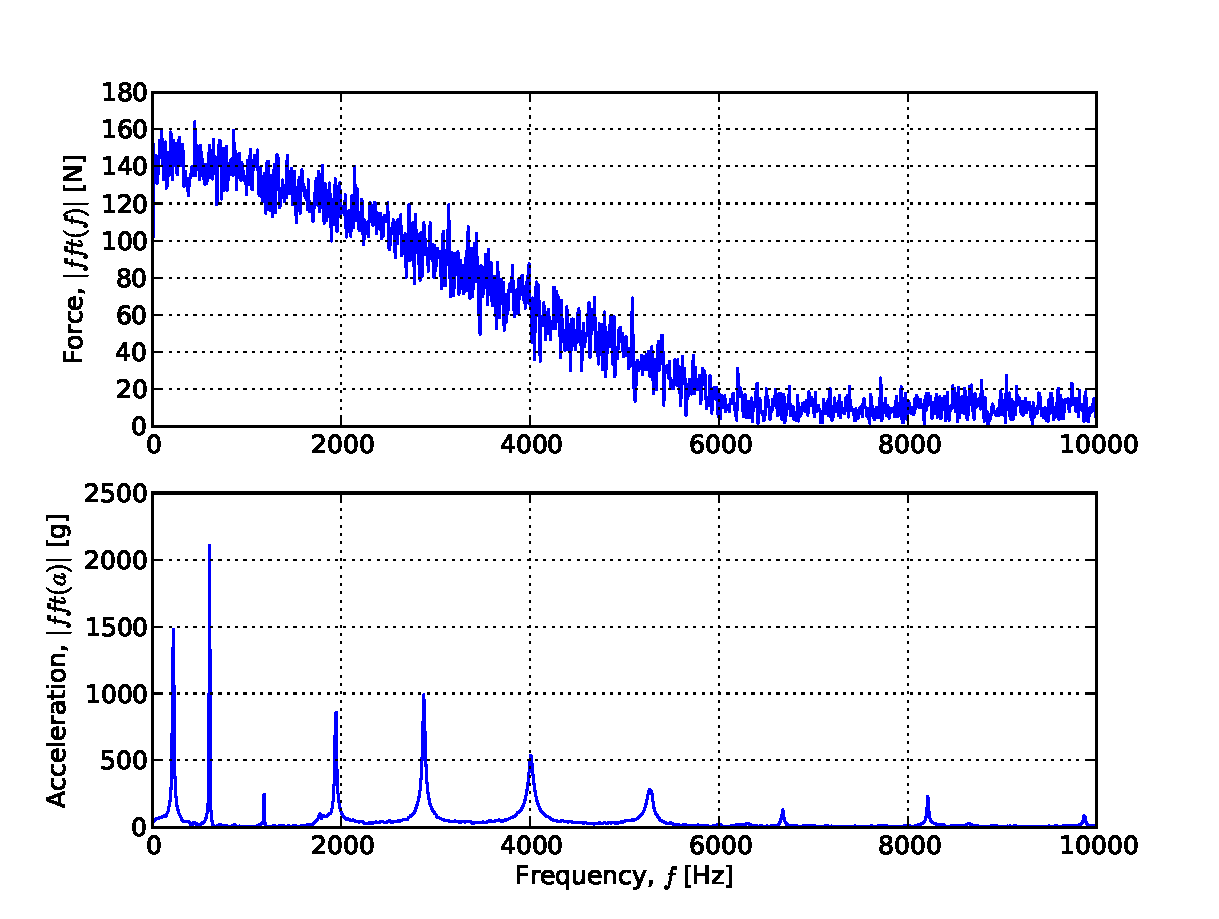
\includegraphics[width=.9\textwidth]{../Example_code/flex_vib_spectre.pdf}
\end{frame}


\begin{frame}{Application à la cloche}
\lstinputlisting{listings/exemple_FFT_cloche.py}
\end{frame}

\begin{frame}{Application à la cloche}
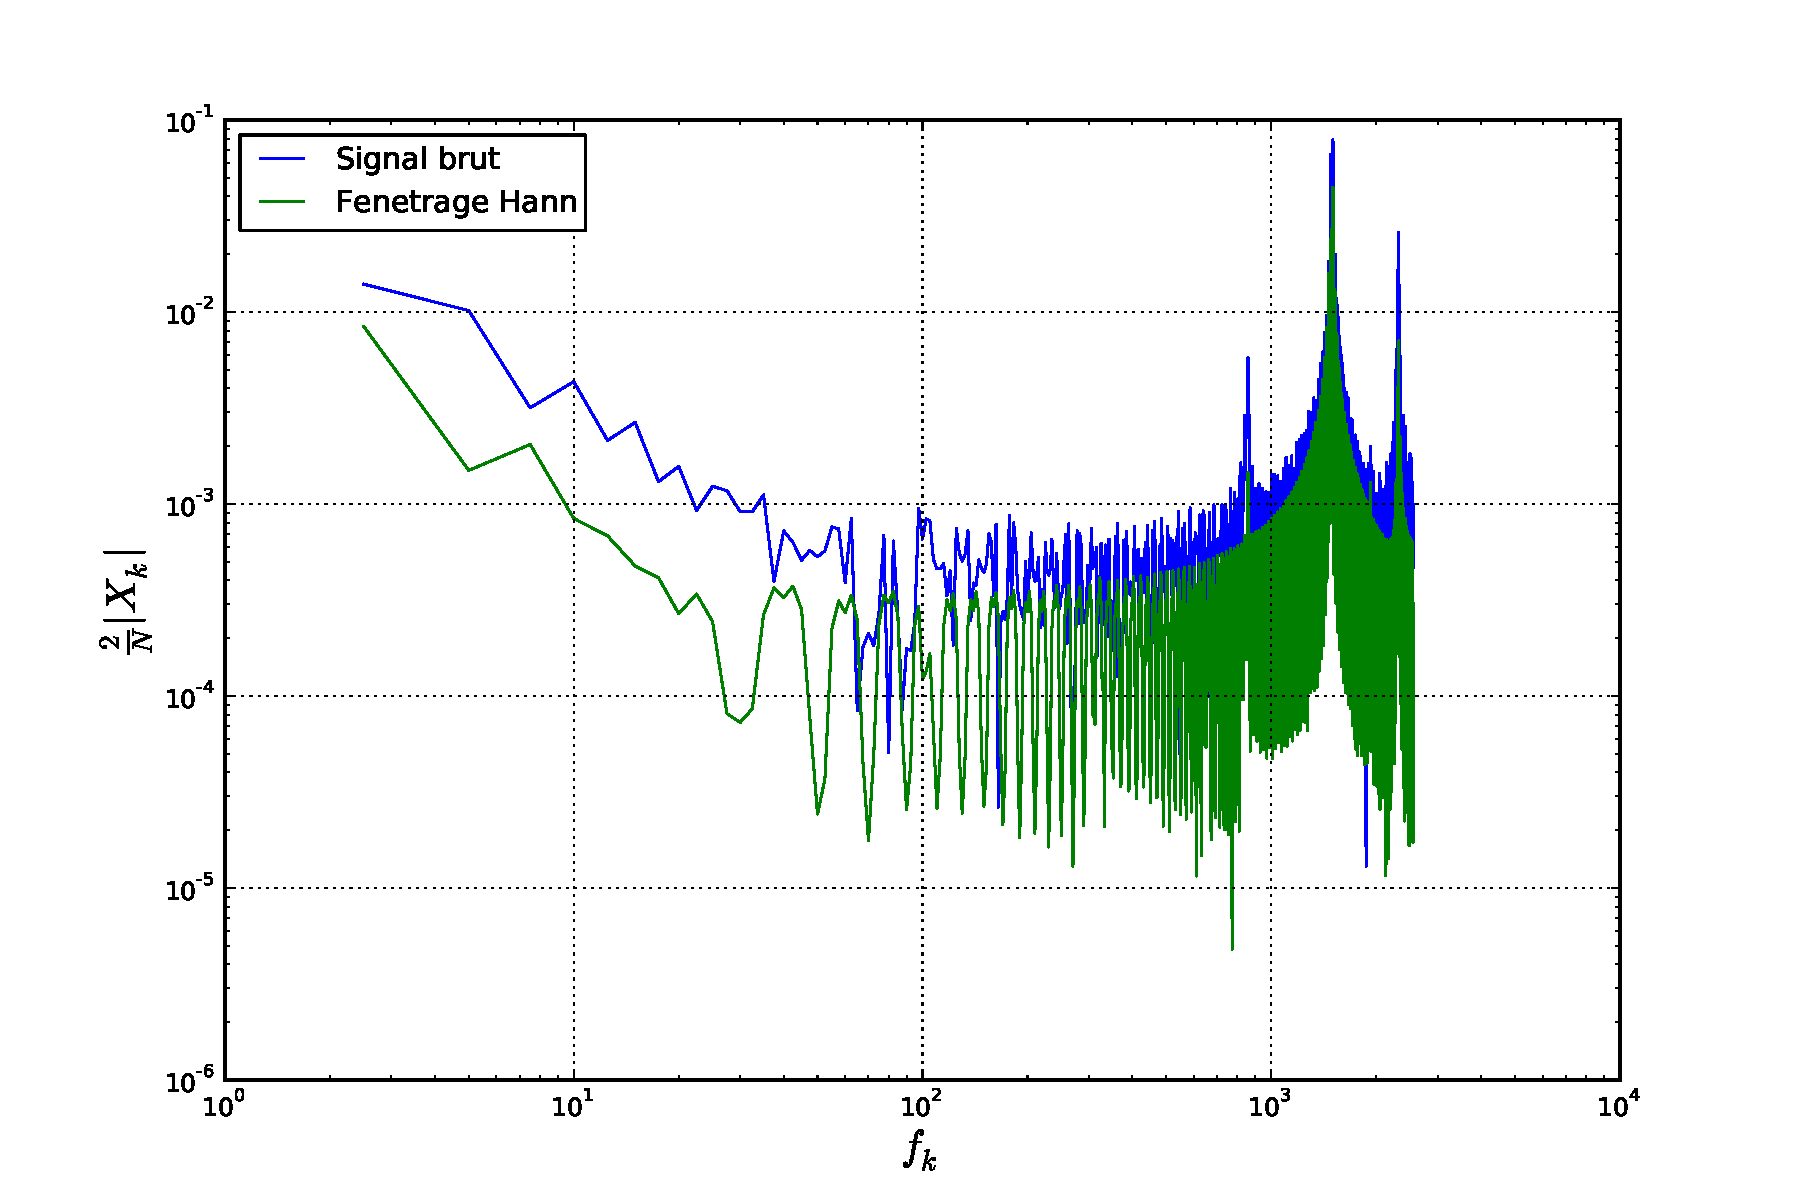
\includegraphics[width=1.\textwidth]{figures/FFT_cloche-log.pdf} \\
\end{frame}

\begin{frame}{Application à la cloche}
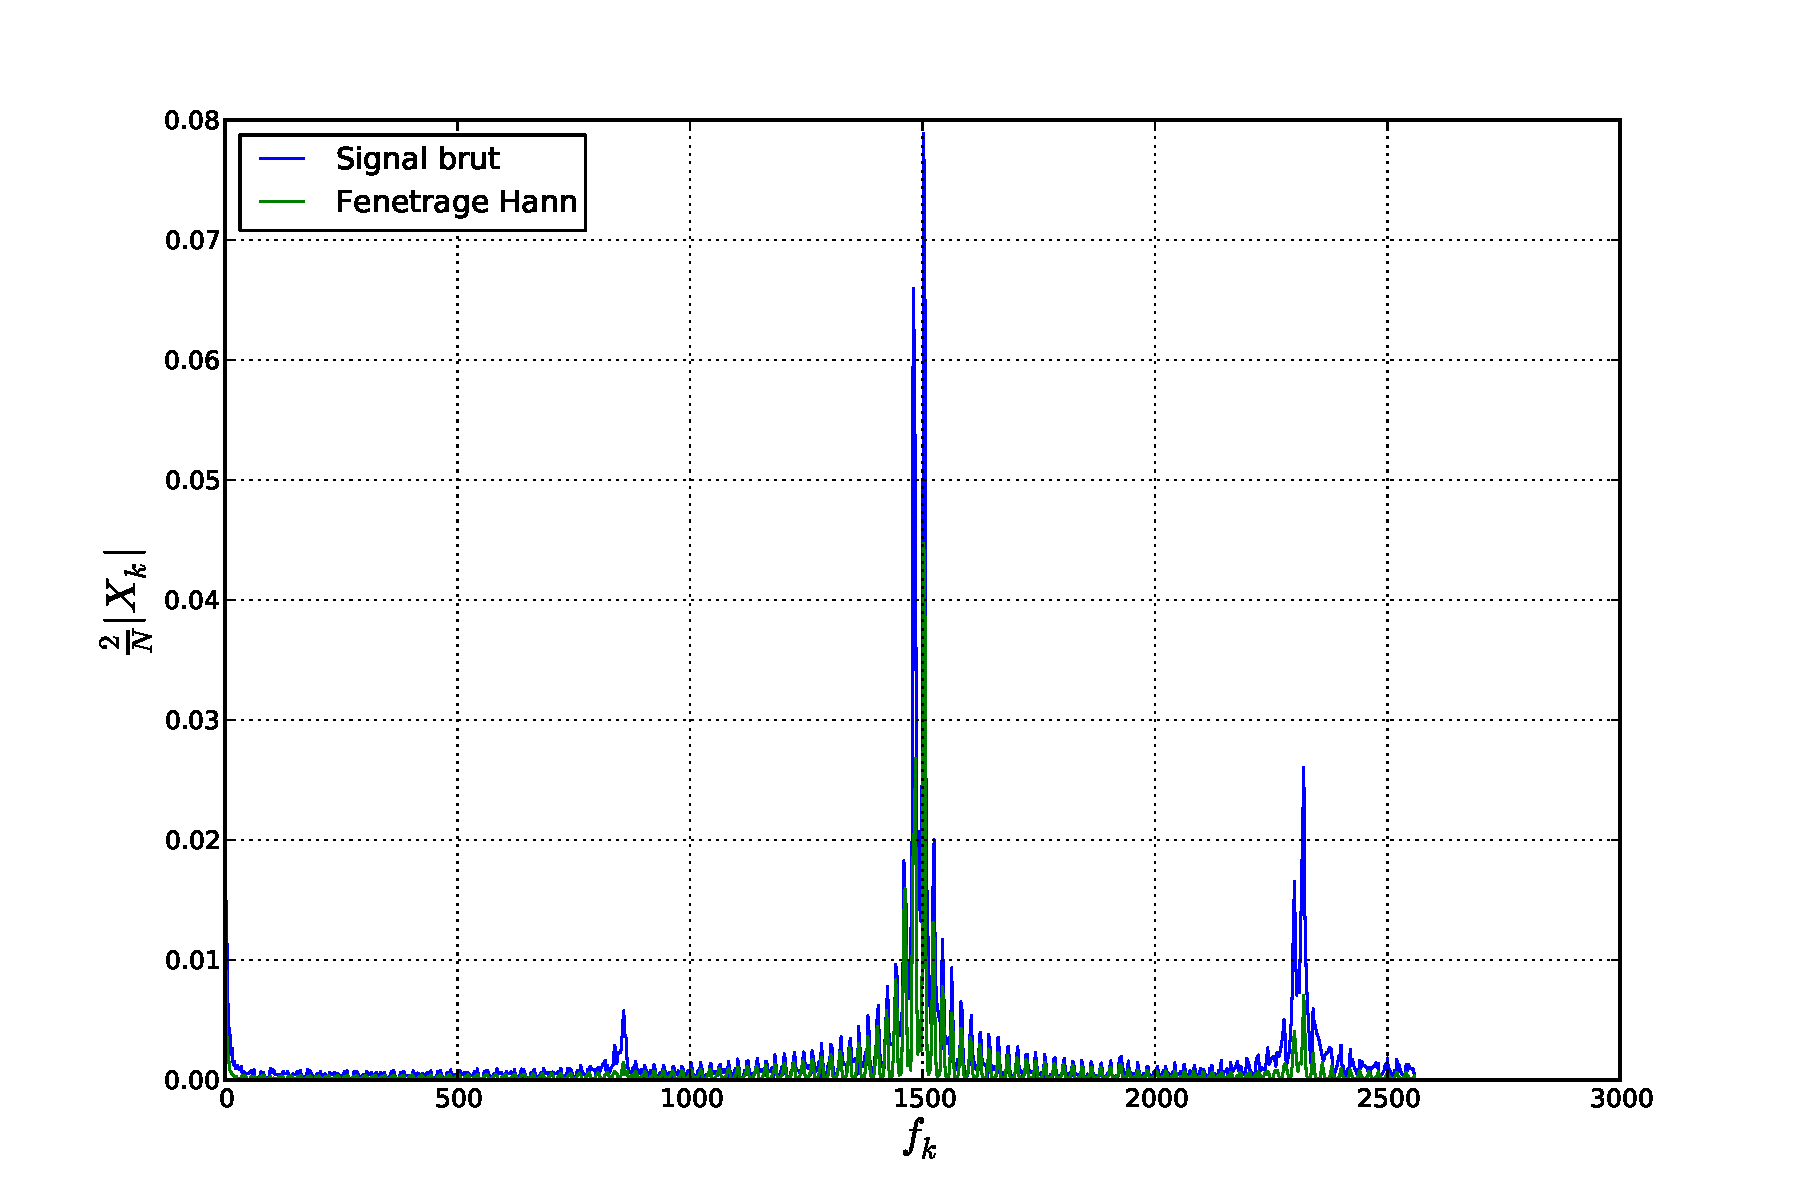
\includegraphics[width=1.\textwidth]{figures/FFT_cloche.pdf} \\
\end{frame}

%\section{Traitement d'images}
%
%\begin{frame}{Séparation des phases dans un alliage SiNb}
%  \begin{columns}
%\column{.35\textwidth}
%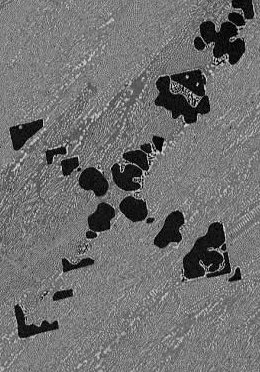
\includegraphics[width=1.\textwidth]{figures/SiNb.png}
%\column{.65\textwidth}
%
%\begin{block}{Image}
%  \begin{itemize}
%  \item 260 x 372 pixels
%  \item 8 bits (256 niveaux de gris).
%  \item $Nb_3Si$ en gris clair et $Nb_3Si_5$ en noir.
%  \item Source: \href{http://www.onera.fr/images-science/materiaux-structures/siliciure-niobium-galerie.php}{Onera}
%  \end{itemize}
%  \end{block}
%\end{columns}
% 
% 
% 
%  \begin{block}{Objectif}
%  \begin{itemize}
%  \item Isoler les deux phases.
%  \item Calculer la proportion de chaque phase.
%  \item Calculer la taille moyenne de chaque dendrite de $Nb_3Si_5$
%  \end{itemize}
%  \end{block}
%  \end{frame}
%
%\begin{frame}{Ouverture d'une image}
%  \begin{columns}
%\column{.45\textwidth}
%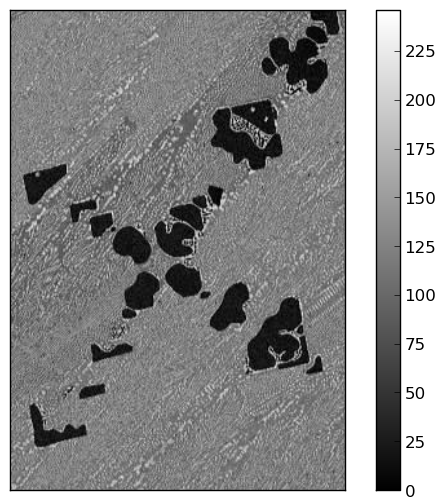
\includegraphics[width=1.\textwidth]{figures/image_original.png}
%\column{.55\textwidth}
%\lstinputlisting[firstline=1,lastline=17,firstnumber=1]{listings/improc/image.py}
%\end{columns}
%\begin{alertblock}{Questions}
%Comment séparer les deux phases ?
%\end{alertblock}
%\end{frame}
%
%\begin{frame}{L'histogramme}
%  \begin{columns}
%\column{.55\textwidth}
%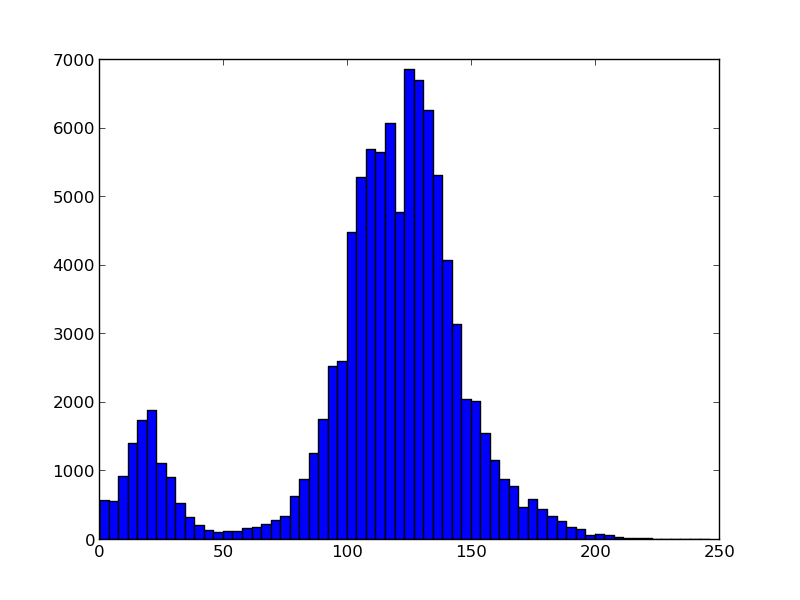
\includegraphics[width=1.\textwidth]{figures/image_hist.png}
%\column{.45\textwidth}
%\lstinputlisting[firstline=19,lastline=24,firstnumber=19]{listings/improc/image.py}
%\end{columns}
%\begin{alertblock}{Questions}
%L'histogramme nous informe-t-il sur les niveaux correspondant aux différentes couleurs ?
%\end{alertblock}
%\end{frame}
%
%
%\begin{frame}{Seuillage}
% \begin{columns}
%\column{.5\textwidth}
%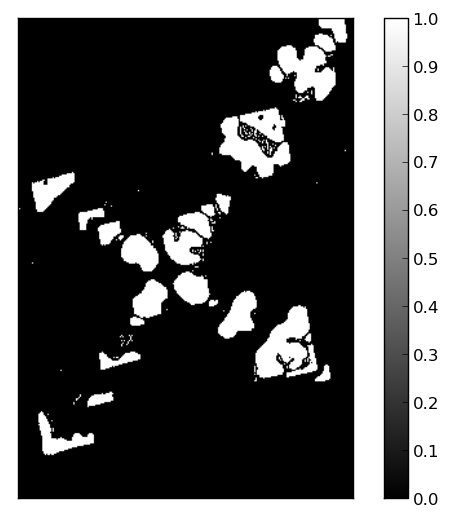
\includegraphics[width=1.\textwidth]{figures/image_threshold.png}
%\column{.5\textwidth}
%\lstinputlisting[firstline=26,lastline=34,firstnumber=26]{listings/improc/image.py}
%\end{columns}
%\begin{alertblock}{Questions}
%L'image seuillée permet-elle de séparer proprement les deux phases ?
%\end{alertblock}
%\end{frame}
%
%\begin{frame}{\'Erosion}
% \begin{columns}
%\column{.5\textwidth}
%\includegraphics[width=1.\textwidth]{figures/image_erosion.png}
%\column{.5\textwidth}
%\lstinputlisting[firstline=37,lastline=48,firstnumber=37]{listings/improc/image.py}
%\end{columns}
%\begin{alertblock}{Questions}
%L'érosion a-t-elle modifié la proportion des deux phases ? comment contrer cet effet ?
%\end{alertblock}
%\end{frame}
%
%\begin{frame}{Dilatation}
% \begin{columns}
%\column{.5\textwidth}
%\includegraphics[width=1.\textwidth]{figures/image_dilation.png}
%\column{.5\textwidth}
%\lstinputlisting[firstline=50,lastline=59,firstnumber=50]{listings/improc/image.py}
%\end{columns}
%\begin{alertblock}{Questions}
%Comment séparer les dendrites ?
%\end{alertblock}
%\end{frame}
%
%\begin{frame}{Labélisation}
% \begin{columns}
%\column{.5\textwidth}
%\includegraphics[width=1.\textwidth]{figures/image_labels.png}
%\column{.5\textwidth}
%\lstinputlisting[firstline=61,lastline=69,firstnumber=61]{listings/improc/image.py}
%\end{columns}
%\begin{alertblock}{Questions}
%Comment compter les dendrites ? 
%\end{alertblock}
%\end{frame}
%
%\begin{frame}{Comptage}
% \begin{columns}
%\column{.5\textwidth}
%\begin{block}{Résultats}
%\begin{itemize}
%\item Proportion de dendrites: $9.6\;\%$
%\item Surface moyenne: $358 \; px \approx \;128 \; \mu m^2$ 
%
%\end{itemize}
%\end{block}
%\column{.5\textwidth}
%\lstinputlisting[firstline=71,lastline=75,firstnumber=71]{listings/improc/image.py}
%\end{columns}
%\begin{alertblock}{Conclusion}
%\begin{itemize}
%\item Outils de traitement quantitatif des images.
%\item Applications très vastes.
%\end{itemize} 
%\end{alertblock}
%\end{frame}
%
%\begin{frame}{Analyse fréquentielle}
% \begin{columns}
%\column{.5\textwidth}
%\includegraphics[width=1.\textwidth]{figures/lapin_original.png}
%\column{.5\textwidth}
%\lstinputlisting[firstline=1,lastline=18,firstnumber=1]{listings/improc/lapin.py}
%\end{columns}
%\begin{alertblock}{Questions}
%Comment utiliser l'analyse fréquentielle pour modifier une image ?
%\end{alertblock}
%\end{frame}
%
%\begin{frame}{FFT 2D}
% \begin{columns}
%\column{.5\textwidth}
%\includegraphics[width=1.\textwidth]{figures/lapin_spectre.png}
%\column{.5\textwidth}
%\lstinputlisting[firstline=20,lastline=28,firstnumber=20]{listings/improc/lapin.py}
%\end{columns}
%\begin{alertblock}{Questions}
%Comment construire un filtre basique à appliquer au spectre du lapin.
%\end{alertblock}
%\end{frame}
%
%\begin{frame}{Filtre passe bas (1/3)}
% \begin{columns}
%\column{.5\textwidth}
%\includegraphics[width=1.\textwidth]{figures/lapin_lowpass.png}
%\column{.5\textwidth}
%\lstinputlisting[firstline=30,lastline=42,firstnumber=30]{listings/improc/lapin.py}
%\end{columns}
%\begin{alertblock}{Questions}
%Comment appliquer ce filtre à notre spectre ?
%\end{alertblock}
%\end{frame}
%
%\begin{frame}{Filtre passe bas (2/3)}
% \begin{columns}
%\column{.5\textwidth}
%\includegraphics[width=1.\textwidth]{figures/lapin_lowpass2.png}
%\column{.5\textwidth}
%\lstinputlisting[firstline=44,lastline=52,firstnumber=44]{listings/improc/lapin.py}
%\end{columns}
%\begin{alertblock}{Questions}
%Quel est le résultat par FFT inverse ?
%\end{alertblock}
%\end{frame}
%
%\begin{frame}{Filtre passe bas (3/3)}
% \begin{columns}
%\column{.5\textwidth}
%\includegraphics[width=1.\textwidth]{figures/lapin_lowpass3.png}
%\column{.5\textwidth}
%\lstinputlisting[firstline=54,lastline=62,firstnumber=54]{listings/improc/lapin.py}
%\end{columns}
%\begin{alertblock}{Questions}
%\begin{itemize}
%\item Trouvez vous la qualité correcte ?
%\item En vous inspirant des exemples 1D, avez vous une idée pour améliorer les choses ?
%\end{itemize}
%\end{alertblock}
%\end{frame}
%
%\begin{frame}{Filtre passe haut}
% \begin{columns}
%\column{.5\textwidth}
%\includegraphics[width=1.\textwidth]{figures/lapin_highpass.png}
%\column{.5\textwidth}
%\lstinputlisting[firstline=64,lastline=78,firstnumber=64]{listings/improc/lapin.py}
%\end{columns}
%\begin{alertblock}{Questions}
%\begin{itemize}
%\item Quelles applications ?
%\end{itemize}
%\end{alertblock}
%\end{frame}

\end{document}


